\documentclass[12pt,a4paper]{article}

% ---------------------------------------------------------------------------
% Dados da capa
% ---------------------------------------------------------------------------
\newcommand{\instituicao}{Universidade do Estado do Amazonas\\[0.2em] Escola Superior de Tecnologia}
\newcommand{\curso}{Engenharia de Computação}
\newcommand{\disciplina}{Processamento Digital de Imagens}
\newcommand{\professor}{Ricardo da Silva Barboza}
\newcommand{\autor}{Henrique da Silva Furtado}
\newcommand{\local}{Manaus-AM}
\newcommand{\data}{9 de novembro de 2026}

\usepackage[T1]{fontenc}
\usepackage[utf8]{inputenc}
\usepackage[brazil]{babel}
\usepackage{lmodern}
\usepackage{microtype}
\usepackage[a4paper,left=3cm,right=2cm,top=3cm,bottom=2cm]{geometry}
\usepackage{graphicx}
\usepackage{float}
\usepackage[font=small,labelfont=bf,justification=centering]{caption}
\usepackage{subcaption}
\usepackage{booktabs}
\usepackage{tabularx}
\usepackage{array}
\newcolumntype{L}{>{\raggedright\arraybackslash}X}
\newcolumntype{P}[1]{>{\raggedright\arraybackslash}p{#1}}
\usepackage{longtable}
\usepackage{amsmath}
\usepackage{amssymb}
\usepackage{xcolor}
\usepackage{listings}
\usepackage{enumitem}
\usepackage{fancyhdr}
\usepackage{titlesec}
\usepackage[hidelinks]{hyperref}

\graphicspath{{../resultados/capturas/}{../resultados/graficos/}{figuras/}}
\setlength{\parskip}{0.4em}
\setlength{\emergencystretch}{3em}
\setlist{itemsep=0.15em, topsep=0.3em}
\titleformat{\section}{\Large\bfseries}{\thesection}{0.6em}{}
\titleformat{\subsection}{\large\bfseries}{\thesubsection}{0.6em}{}

\setlength{\headheight}{14pt}
\pagestyle{fancy}
\fancyhf{}
\fancyhead[L]{\small Atividade 3 -- Desempenho de CPU e GPU com OpenGL}
\fancyhead[R]{\small\thepage}
\renewcommand{\headrulewidth}{0.4pt}

\newcommand{\code}[1]{\texttt{\detokenize{#1}}}
% Gerado por tools/graficos.py -- nao editar
\newcommand{\limVboA}{82.463.760}
\newcommand{\limMVboA}{82,5}
\newcommand{\fpsVboA}{59,8}
\newcommand{\gpuVboA}{95}
\newcommand{\thrVboA}{8}
\newcommand{\cpuVboA}{0,7}
\newcommand{\acimaVboA}{80.155.664}
\newcommand{\fpsAcimaVboA}{63,2}
\newcommand{\pontosVboA}{15}
\newcommand{\fpsMenorVboA}{1.729}
\newcommand{\limVboB}{82.463.760}
\newcommand{\limMVboB}{82,5}
\newcommand{\fpsVboB}{58,5}
\newcommand{\gpuVboB}{95}
\newcommand{\thrVboB}{9}
\newcommand{\cpuVboB}{0,7}
\newcommand{\acimaVboB}{80.155.664}
\newcommand{\fpsAcimaVboB}{62,8}
\newcommand{\pontosVboB}{15}
\newcommand{\fpsMenorVboB}{1.719}
\newcommand{\limVboC}{82.463.760}
\newcommand{\limMVboC}{82,5}
\newcommand{\fpsVboC}{58,4}
\newcommand{\gpuVboC}{97}
\newcommand{\thrVboC}{10}
\newcommand{\cpuVboC}{0,7}
\newcommand{\acimaVboC}{80.155.664}
\newcommand{\fpsAcimaVboC}{62,9}
\newcommand{\pontosVboC}{15}
\newcommand{\fpsMenorVboC}{1.640}
\newcommand{\limVboD}{82.463.760}
\newcommand{\limMVboD}{82,5}
\newcommand{\fpsVboD}{59,3}
\newcommand{\gpuVboD}{97}
\newcommand{\thrVboD}{10}
\newcommand{\cpuVboD}{0,7}
\newcommand{\acimaVboD}{80.155.664}
\newcommand{\fpsAcimaVboD}{63,8}
\newcommand{\pontosVboD}{15}
\newcommand{\fpsMenorVboD}{1.625}
\newcommand{\limVboE}{82.463.760}
\newcommand{\limMVboE}{82,5}
\newcommand{\fpsVboE}{57,9}
\newcommand{\gpuVboE}{97}
\newcommand{\thrVboE}{9}
\newcommand{\cpuVboE}{0,7}
\newcommand{\acimaVboE}{80.155.664}
\newcommand{\fpsAcimaVboE}{62,0}
\newcommand{\pontosVboE}{15}
\newcommand{\fpsMenorVboE}{1.659}
\newcommand{\limVboF}{82.463.760}
\newcommand{\limMVboF}{82,5}
\newcommand{\fpsVboF}{58,8}
\newcommand{\gpuVboF}{95}
\newcommand{\thrVboF}{8}
\newcommand{\cpuVboF}{0,6}
\newcommand{\acimaVboF}{80.155.664}
\newcommand{\fpsAcimaVboF}{62,5}
\newcommand{\pontosVboF}{15}
\newcommand{\fpsMenorVboF}{1.543}
\newcommand{\limImedA}{524.304}
\newcommand{\limMImedA}{0,5}
\newcommand{\fpsImedA}{57,6}
\newcommand{\gpuImedA}{23}
\newcommand{\thrImedA}{99}
\newcommand{\cpuImedA}{5,0}
\newcommand{\acimaImedA}{501.776}
\newcommand{\fpsAcimaImedA}{60,8}
\newcommand{\pontosImedA}{10}
\newcommand{\fpsMenorImedA}{557}
\newcommand{\limImedB}{524.304}
\newcommand{\limMImedB}{0,5}
\newcommand{\fpsImedB}{56,8}
\newcommand{\gpuImedB}{23}
\newcommand{\thrImedB}{98}
\newcommand{\cpuImedB}{5,0}
\newcommand{\acimaImedB}{501.776}
\newcommand{\fpsAcimaImedB}{60,5}
\newcommand{\pontosImedB}{10}
\newcommand{\fpsMenorImedB}{598}
\newcommand{\limImedC}{501.776}
\newcommand{\limMImedC}{0,5}
\newcommand{\fpsImedC}{59,7}
\newcommand{\gpuImedC}{23}
\newcommand{\thrImedC}{99}
\newcommand{\cpuImedC}{5,0}
\newcommand{\acimaImedC}{479.760}
\newcommand{\fpsAcimaImedC}{62,8}
\newcommand{\pontosImedC}{10}
\newcommand{\fpsMenorImedC}{605}
\newcommand{\limImedD}{501.776}
\newcommand{\limMImedD}{0,5}
\newcommand{\fpsImedD}{59,8}
\newcommand{\gpuImedD}{23}
\newcommand{\thrImedD}{98}
\newcommand{\cpuImedD}{4,9}
\newcommand{\acimaImedD}{479.760}
\newcommand{\fpsAcimaImedD}{60,8}
\newcommand{\pontosImedD}{10}
\newcommand{\fpsMenorImedD}{613}
\newcommand{\limImedE}{501.776}
\newcommand{\limMImedE}{0,5}
\newcommand{\fpsImedE}{58,3}
\newcommand{\gpuImedE}{20}
\newcommand{\thrImedE}{97}
\newcommand{\cpuImedE}{4,9}
\newcommand{\acimaImedE}{479.760}
\newcommand{\fpsAcimaImedE}{61,5}
\newcommand{\pontosImedE}{10}
\newcommand{\fpsMenorImedE}{612}
\newcommand{\limImedF}{501.776}
\newcommand{\limMImedF}{0,5}
\newcommand{\fpsImedF}{57,5}
\newcommand{\gpuImedF}{20}
\newcommand{\thrImedF}{98}
\newcommand{\cpuImedF}{4,9}
\newcommand{\acimaImedF}{479.760}
\newcommand{\fpsAcimaImedF}{60,9}
\newcommand{\pontosImedF}{10}
\newcommand{\fpsMenorImedF}{609}
\newcommand{\limObjA}{5.981.200}
\newcommand{\limMObjA}{6,0}
\newcommand{\fpsObjA}{59,4}
\newcommand{\gpuObjA}{18}
\newcommand{\thrObjA}{97}
\newcommand{\cpuObjA}{4,9}
\newcommand{\acimaObjA}{5.751.824}
\newcommand{\fpsAcimaObjA}{61,9}
\newcommand{\pontosObjA}{12}
\newcommand{\fpsMenorObjA}{1.611}
\newcommand{\limObjF}{5.751.824}
\newcommand{\limMObjF}{5,8}
\newcommand{\fpsObjF}{59,8}
\newcommand{\gpuObjF}{19}
\newcommand{\thrObjF}{99}
\newcommand{\cpuObjF}{4,9}
\newcommand{\acimaObjF}{5.522.448}
\newcommand{\fpsAcimaObjF}{62,1}
\newcommand{\pontosObjF}{12}
\newcommand{\fpsMenorObjF}{1.718}
\newcommand{\limIntA}{12.351.504}
\newcommand{\limMIntA}{12,4}
\newcommand{\fpsIntA}{58,8}
\newcommand{\gpuIntA}{99}
\newcommand{\thrIntA}{15}
\newcommand{\cpuIntA}{0,9}
\newcommand{\acimaIntA}{11.906.064}
\newcommand{\fpsAcimaIntA}{60,5}
\newcommand{\pontosIntA}{10}
\newcommand{\fpsMenorIntA}{320}
\newcommand{\limIntB}{12.351.504}
\newcommand{\limMIntB}{12,4}
\newcommand{\fpsIntB}{58,5}
\newcommand{\gpuIntB}{98}
\newcommand{\thrIntB}{14}
\newcommand{\cpuIntB}{0,8}
\newcommand{\acimaIntB}{11.906.064}
\newcommand{\fpsAcimaIntB}{60,5}
\newcommand{\pontosIntB}{10}
\newcommand{\fpsMenorIntB}{320}
\newcommand{\limIntC}{12.351.504}
\newcommand{\limMIntC}{12,4}
\newcommand{\fpsIntC}{58,6}
\newcommand{\gpuIntC}{98}
\newcommand{\thrIntC}{14}
\newcommand{\cpuIntC}{0,9}
\newcommand{\acimaIntC}{11.906.064}
\newcommand{\fpsAcimaIntC}{60,6}
\newcommand{\pontosIntC}{10}
\newcommand{\fpsMenorIntC}{326}
\newcommand{\limIntD}{11.906.064}
\newcommand{\limMIntD}{11,9}
\newcommand{\fpsIntD}{59,6}
\newcommand{\gpuIntD}{98}
\newcommand{\thrIntD}{15}
\newcommand{\cpuIntD}{0,9}
\newcommand{\acimaIntD}{11.468.816}
\newcommand{\fpsAcimaIntD}{62,3}
\newcommand{\pontosIntD}{10}
\newcommand{\fpsMenorIntD}{319}
\newcommand{\limIntE}{11.906.064}
\newcommand{\limMIntE}{11,9}
\newcommand{\fpsIntE}{59,1}
\newcommand{\gpuIntE}{96}
\newcommand{\thrIntE}{15}
\newcommand{\cpuIntE}{0,9}
\newcommand{\acimaIntE}{11.468.816}
\newcommand{\fpsAcimaIntE}{61,0}
\newcommand{\pontosIntE}{10}
\newcommand{\fpsMenorIntE}{316}
\newcommand{\limIntF}{12.351.504}
\newcommand{\limMIntF}{12,4}
\newcommand{\fpsIntF}{58,7}
\newcommand{\gpuIntF}{99}
\newcommand{\thrIntF}{14}
\newcommand{\cpuIntF}{0,8}
\newcommand{\acimaIntF}{11.906.064}
\newcommand{\fpsAcimaIntF}{60,6}
\newcommand{\pontosIntF}{10}
\newcommand{\fpsMenorIntF}{320}


\definecolor{fundocodigo}{RGB}{248,248,248}
\definecolor{comentario}{RGB}{0,110,0}
\definecolor{palavra}{RGB}{0,0,170}
\definecolor{cadeia}{RGB}{160,40,0}
% Código-fonte SEM numeração de linhas (pode ser copiado e compilado diretamente)
\lstset{
  basicstyle=\ttfamily\scriptsize,
  backgroundcolor=\color{fundocodigo},
  frame=single, rulecolor=\color{black!25},
  numbers=none,
  keywordstyle=\color{palavra}\bfseries,
  commentstyle=\color{comentario}\itshape,
  stringstyle=\color{cadeia},
  breaklines=true, breakatwhitespace=false,
  showstringspaces=false, tabsize=4, columns=fullflexible, keepspaces=true,
  upquote=true,
  literate={á}{{\'a}}1 {Á}{{\'A}}1 {â}{{\^a}}1 {Â}{{\^A}}1 {ã}{{\~a}}1 {à}{{\`a}}1
           {é}{{\'e}}1 {É}{{\'E}}1 {ê}{{\^e}}1 {Ê}{{\^E}}1 {í}{{\'i}}1 {Í}{{\'I}}1
           {ó}{{\'o}}1 {Ó}{{\'O}}1 {ô}{{\^o}}1 {õ}{{\~o}}1 {ú}{{\'u}}1 {Ú}{{\'U}}1
           {ç}{{\c{c}}}1 {Ç}{{\c{C}}}1 {×}{{$\times$}}1 {≥}{{$\geq$}}1 {≤}{{$\leq$}}1
           {—}{{---}}1 {–}{{--}}1 {−}{{-}}1 {°}{{$^\circ$}}1 {±}{{$\pm$}}1 {º}{{\textordmasculine}}1
}

\begin{document}

% ===========================================================================
% CAPA
% ===========================================================================
\begin{titlepage}
\centering
{\large\bfseries \MakeUppercase{\instituicao}\par}
{\large \curso\par}
{\large Disciplina: \disciplina\par}
\vfill
{\LARGE\bfseries Relatório Técnico -- Atividade 3\par}
\vspace{0.8cm}
{\Large Análise de desempenho de CPU e GPU utilizando OpenGL:\\[0.2em]
quantidade de polígonos, iluminação, texturas e o limite de 60 FPS\par}
\vfill
{\large \autor\par}
\vspace{1.5cm}
\begin{flushright}
\begin{minipage}{0.55\textwidth}
Relatório técnico apresentado à disciplina de \disciplina, contendo a aplicação gráfica em
C++/OpenGL/FreeGLUT, a metodologia e os resultados das medições de desempenho, a investigação
dos gargalos e o código-fonte completo em anexo.\\[0.6em]
Professor(a): \professor
\end{minipage}
\end{flushright}
\vfill
{\large \local\\ \data\par}
\end{titlepage}

\pagenumbering{roman}
\tableofcontents
\newpage
\listoffigures
\listoftables
\newpage
\pagenumbering{arabic}

% ===========================================================================
\section{Objetivos}
% ===========================================================================

\textbf{Objetivo geral.} Investigar experimentalmente o desempenho de uma aplicação gráfica
em C++ com OpenGL e FreeGLUT, analisando a influência da quantidade de polígonos, da
iluminação e das texturas sobre a taxa de quadros por segundo (FPS) e sobre a utilização da
CPU e da GPU, e determinar, para cada uma das seis configurações gráficas exigidas, a
quantidade de polígonos a partir da qual o FPS \emph{médio} fica abaixo de 60.

\noindent\textbf{Objetivos específicos.}
\begin{itemize}
  \item Caracterizar o hardware e identificar qual GPU executa a aplicação OpenGL num
        notebook com GPU integrada (Intel Arc) e dedicada (NVIDIA GeForce RTX 4060 Laptop).
  \item Desenvolver uma única aplicação com cena original e animação contínua, com controle
        da quantidade de polígonos, iluminação omnidirecional e \emph{spot}, texturas e
        contagem exata dos triângulos renderizados por quadro.
  \item Medir FPS, tempo por quadro, tempo de GPU, tempo de CPU e utilização de CPU, GPU,
        memória, potência e clock, com protocolo repetível (3 repetições de 10 s após
        estabilização, V-Sync desligado).
  \item Localizar, por varredura progressiva e refino por bisseção, a menor quantidade testada
        de triângulos com FPS médio inferior a 60 nas configurações A a F.
  \item Identificar o gargalo (\emph{bottleneck}) de cada situação, distinguindo conclusões
        sustentadas pelos dados de hipóteses, e avaliar o efeito da iluminação e das texturas.
\end{itemize}

% ===========================================================================
\section{Introdução teórica}
% ===========================================================================

\subsection{Quadros por segundo e tempo por quadro}

Uma aplicação gráfica interativa produz uma sequência de imagens (\emph{quadros}). A
\textbf{taxa de quadros} é $\text{FPS} = n/\Delta t$, o número de quadros $n$ concluídos num
intervalo $\Delta t$. A grandeza equivalente e mais útil para análise é o \textbf{tempo por
quadro} $t_q = 1000/\text{FPS}$ (ms), porque os custos das etapas se \emph{somam} em tempo, e
não em FPS. O limite de 60 FPS corresponde a um orçamento de $1000/60 \approx 16{,}7$~ms por
quadro, o valor típico da taxa de atualização de monitores e uma referência comum de fluidez
\cite{akenine}. Como $t_q$ e FPS são inversos, uma mesma economia de tempo (por exemplo,
1~ms) vale muito mais FPS quando o FPS é alto do que quando é baixo; por isso as médias deste
trabalho são calculadas sobre quadros contados num intervalo longo (10~s), e não sobre valores
instantâneos.

O \textbf{V-Sync} (sincronismo vertical) faz a troca de \emph{buffers} esperar o retraço do
monitor, limitando o FPS à frequência de atualização (60 ou 120~Hz). Uma leitura de 60~FPS com
V-Sync ligado não revela a capacidade excedente; por isso os testes desligam o V-Sync
(\code{wglSwapIntervalEXT(0)}).

\subsection{O pipeline gráfico: o papel da CPU e da GPU}

No OpenGL, a aplicação, executada na \textbf{CPU}, prepara o estado (matrizes, texturas,
programas de \emph{shader}) e emite comandos de desenho. O \emph{driver} traduz esses comandos
e os coloca numa fila consumida pela \textbf{GPU}, que executa o \emph{pipeline} gráfico
\cite{akenine,redbook}:
\begin{enumerate}
  \item \textbf{processamento de vértices}: o \emph{vertex shader} transforma cada vértice
        (matrizes de modelagem, visualização e projeção) e calcula atributos;
  \item \textbf{montagem e rasterização}: os triângulos são montados, recortados, descartados
        se estiverem de costas (\emph{back-face culling}) e convertidos em fragmentos (pixels);
  \item \textbf{processamento de fragmentos}: o \emph{fragment shader} calcula a cor de cada
        fragmento (iluminação, textura), seguido do teste de profundidade e da escrita no
        \emph{framebuffer}.
\end{enumerate}
CPU e GPU trabalham em paralelo, como uma linha de produção: enquanto a GPU desenha o quadro
$k$, a CPU já prepara o quadro $k+1$. Por isso o tempo por quadro é aproximadamente o
\textbf{máximo} (e não a soma) entre o tempo de CPU e o tempo de GPU de cada quadro. A etapa
mais lenta determina o FPS: é o \textbf{gargalo} (\emph{bottleneck}) \cite{akenine,nvidiaperf}.

\subsection{Gargalos}

\begin{itemize}
  \item \textbf{Gargalo de CPU}: a GPU fica ociosa esperando comandos. Ocorre quando o custo de
        \emph{emitir} o trabalho (chamadas de função, validação de estado pelo \emph{driver},
        uma chamada de desenho por objeto) é maior que o custo de \emph{executá-lo}. Como a
        emissão de comandos OpenGL de um contexto é essencialmente sequencial, o gargalo de CPU
        costuma ser \textbf{uma única thread saturada}, com utilização total da CPU baixa: em
        um processador com 22 threads lógicas, uma thread a 100\% corresponde a apenas
        $100/22 \approx 4{,}5\%$ da CPU inteira.
  \item \textbf{Gargalo de GPU}: a CPU espera a GPU (tipicamente bloqueada na troca de
        \emph{buffers}). Pode estar no processamento de vértices (muitos vértices), na
        rasterização (muitos triângulos minúsculos), nos fragmentos (muitos pixels, \emph{shaders}
        caros, texturas) ou na largura de banda de memória.
  \item \textbf{Outros limites}: potência e temperatura (a GPU reduz o clock ao atingir o limite
        de potência ou térmico), sincronização (V-Sync, esperas do \emph{driver}), transferência
        de dados entre CPU e GPU e, em notebooks com duas GPUs, a cópia do quadro da GPU dedicada
        para a integrada, que é a ligada à tela.
\end{itemize}
Utilização próxima de 100\% é um \emph{indício}, não uma prova: uma thread pode aparecer ocupada
porque está em espera ativa (\emph{busy-wait}) pela GPU, e uma GPU pode estar ``100\% ocupada''
apenas no sentido de ter sempre algum trabalho na fila. Este trabalho, por isso, cruza três tipos
de evidência: (i) utilização dos recursos, (ii) decomposição do tempo do quadro (tempo de GPU
medido pela própria GPU \emph{versus} tempo efetivo de CPU) e (iii) a forma como o FPS escala
quando se muda a carga de um recurso específico.

\subsection{Iluminação}

O modelo de reflexão usado é o de \textbf{Blinn-Phong} \cite{blinn,phong}, calculado
\emph{por fragmento}:
\begin{equation}
  \mathbf{c} = \mathbf{k}_d \odot \left(\mathbf{a} + f_{at}\, f_{spot}\, \max(\mathbf{n}\cdot\mathbf{l},0)\, \mathbf{i}_L\right)
             + k_s\, f_{at}\, f_{spot}\, \max(\mathbf{n}\cdot\mathbf{h},0)^{\alpha}\, \mathbf{i}_L,
  \qquad \mathbf{h} = \frac{\mathbf{l}+\mathbf{v}}{\lVert\mathbf{l}+\mathbf{v}\rVert},
  \label{eq:blinn}
\end{equation}
em que $\mathbf{k}_d$ é a cor difusa do material (modulada pela textura), $\mathbf{a}$ a luz
ambiente, $\mathbf{n}$ a normal, $\mathbf{l}$ a direção para a luz, $\mathbf{v}$ a direção para o
observador, $\alpha=48$ o expoente especular e $\mathbf{i}_L$ a cor da luz. A atenuação com a
distância $d$ é $f_{at}=1/(1+0{,}010\,d+0{,}002\,d^2)$.
\begin{itemize}
  \item \textbf{Luz omnidirecional} (\emph{point light}): emite igualmente em todas as direções a
        partir de um ponto; $f_{spot}=1$.
  \item \textbf{Luz spot} (\emph{spotlight}): emite dentro de um cone de eixo $\mathbf{s}$. Com
        $\theta$ o ângulo entre $-\mathbf{l}$ e $\mathbf{s}$,
        $f_{spot}=\mathrm{smoothstep}(\cos\theta_{ext},\cos\theta_{int},\cos\theta)$, com
        $\theta_{int}=18^\circ$ e $\theta_{ext}=26^\circ$ (borda suave).
\end{itemize}
Calcular a iluminação por fragmento custa operações proporcionais ao número de pixels cobertos;
no OpenGL de \emph{pipeline} fixo ela seria calculada por vértice (modelo de Gouraud), o que
torna o \emph{spot} visualmente pobre em superfícies com poucos vértices.

\subsection{Texturas}

Uma textura é uma imagem amostrada a cada fragmento por coordenadas $(u,v)$. Para evitar
\emph{aliasing} ao reduzir a imagem, usam-se \textbf{mipmaps} (versões reduzidas pré-calculadas)
com filtragem \textbf{trilinear} (interpolação entre 8 texels de dois níveis) e, aqui, também
\textbf{anisotrópica} 8x, que amostra mais texels quando a superfície é vista em ângulo rasante
\cite{akenine,williams}. O custo de uma textura está nos acessos à memória por fragmento;
a cache de texturas da GPU torna esse custo baixo quando os acessos são coerentes.

\subsection{Modos de envio da geometria}

\begin{itemize}
  \item \textbf{Modo imediato} (\code{glBegin}/\code{glVertex}/\code{glEnd}): cada atributo de cada
        vértice é uma chamada de função, a cada quadro. Todo o trabalho de enviar a geometria
        recai sobre a CPU (e o barramento). Foi removido do perfil \emph{core} do OpenGL 3.1.
  \item \textbf{Vertex Buffer Objects} (VBO): vértices e índices ficam na memória de vídeo e um
        único \code{glDrawElements} desenha milhares ou milhões de triângulos \cite{glspec}.
\end{itemize}

% ===========================================================================
\section{Ambiente de desenvolvimento}
% ===========================================================================

\begin{table}[H]
\centering
\caption{Ferramentas e bibliotecas utilizadas.}
\label{tab:ambiente}
\small
\begin{tabularx}{\textwidth}{l L}
\toprule
Item & Versão / observação \\
\midrule
Linguagem & C++17 \\
Compilador & Microsoft Visual C++ 14.44 (Visual Studio 2022), x64, Release (\code{/O2}) \\
Sistema de compilação & CMake 3.31 (gerador ``Visual Studio 17 2022''), script \code{build.bat} \\
Janelas e entrada & FreeGLUT 3.8.0 \\
API gráfica & OpenGL 4.6 em perfil de compatibilidade; \emph{shaders} GLSL 1.20 \\
Extensões OpenGL & carregador próprio (\code{gl_ext.cpp}) via \code{glutGetProcAddress}, sem GLEW/GLAD \\
Monitoramento & API Win32 (PDH, Toolhelp32, DXGI) e NVML (NVIDIA Management Library), \\
               & carregada dinamicamente; Gerenciador de Tarefas para conferência visual \\
Capturas de tela & OpenCV 4.14.0 (opcional, só para gravar PNG) \\
Gráficos e tabelas & Python 3.14 com matplotlib 3.11 (\code{tools/graficos.py}) \\
Relatório & \LaTeX\ (MiKTeX, \code{pdflatex}) \\
\bottomrule
\end{tabularx}
\end{table}

Todo o projeto é um único CMake com os mesmos arquivos-fonte, compilado em dois executáveis
que diferem só numa definição de compilação: \code{desempenho_gl} exporta o símbolo
\code{NvOptimusEnablement}, que pede ao \emph{driver} que crie o contexto OpenGL na GPU NVIDIA
dedicada (usado em todos os experimentos principais), e \code{desempenho_gl_integrada} não o
exporta, deixando o Windows escolher a GPU (no equipamento usado, a integrada). Isso permitiu
comparar as duas GPUs sem alterar o código.

% ===========================================================================
\section{Caracterização do hardware}
% ===========================================================================

Os dados da Tabela~\ref{tab:hardware} foram obtidos pela própria aplicação (opção
\code{--info}, que consulta o registro do Windows, DXGI, NVML e \code{glGetString}) e conferidos
no Gerenciador de Tarefas e com \code{nvidia-smi}.

\begin{table}[H]
\centering
\caption{Caracterização do hardware e do software de sistema.}
\label{tab:hardware}
\small
\begin{tabularx}{\textwidth}{l L}
\toprule
Componente & Descrição \\
\midrule
Equipamento & Notebook Dell Inspiron 16 Plus 7640, ligado à tomada (bateria 100\%), plano de energia ``Equilibrado'' \\
CPU & Intel Core Ultra 7 155H (Meteor Lake): 16 núcleos (6 de desempenho, 8 de eficiência, 2 de baixo consumo) e 22 threads lógicas; até 4,8~GHz \\
Memória RAM & 32~GB (2 $\times$ 16~GB) DDR5-5600 (31,5~GB visíveis) \\
GPU dedicada & NVIDIA GeForce RTX 4060 Laptop GPU (Ada Lovelace), 8~GB GDDR6 dedicados (7\,956~MB informados pelo DXGI), \emph{driver} 621.01, limite de potência observado $\approx$ 60~W \\
GPU integrada & Intel Arc Graphics (Xe-LPG, 8 núcleos Xe), 128~MB dedicados + memória compartilhada da RAM (até 18~GB), \emph{driver} 32.0.101.8860 \\
Tela & 2560 $\times$ 1600, 120~Hz, ligada à GPU integrada (arquitetura NVIDIA Optimus) \\
Sistema operacional & Windows 11 Pro 25H2 (build 26200), 64 bits \\
OpenGL (GPU dedicada) & \code{GL_VERSION} = 4.6.0 NVIDIA 621.01; \code{GL_RENDERER} = NVIDIA GeForce RTX 4060 Laptop GPU/PCIe/SSE2; GLSL 4.60 \\
OpenGL (GPU integrada) & \code{GL_VERSION} = 4.6.0 - Build 32.0.101.8860; \code{GL_RENDERER} = Intel(R) Arc(TM) Graphics \\
Recursos usados & consultas de tempo da GPU (\code{GL_TIME_ELAPSED}), filtragem anisotrópica, controle do V-Sync (\code{WGL_EXT_swap_control}) \\
\bottomrule
\end{tabularx}
\end{table}

\subsection{Qual GPU executa a aplicação?}

O equipamento possui duas GPUs. A tela está ligada à GPU integrada; a GPU NVIDIA renderiza e
copia o quadro pronto para a integrada, que o compõe na área de trabalho (Optimus). Três
evidências independentes identificam a GPU que executa a aplicação:
\begin{enumerate}
  \item \code{glGetString(GL_RENDERER)} informa o dispositivo que atende ao contexto OpenGL:
        ``NVIDIA GeForce RTX 4060 Laptop GPU'' no executável principal e ``Intel(R) Arc(TM)
        Graphics'' no executável \code{_integrada};
  \item os contadores de desempenho do Windows \code{\GPU Engine(*)\Utilization Percentage},
        a mesma fonte do Gerenciador de Tarefas, trazem no nome de cada instância o \emph{pid} do
        processo, o LUID do adaptador e o tipo de motor (3D, cópia, vídeo\dots). A aplicação
        filtra as instâncias pelo seu próprio \emph{pid} e associa o LUID ao nome do adaptador
        via DXGI. Durante os testes com o executável principal, o motor 3D do processo esteve
        ativo apenas na NVIDIA (0\% de 3D na Intel);
  \item a NVML mostra potência, clock e utilização da NVIDIA subindo com a carga.
\end{enumerate}
Sim, é possível acompanhar separadamente o percentual de cada GPU: o Gerenciador de Tarefas
mostra ``GPU 0'' (NVIDIA) e ``GPU 1'' (Intel) e a aplicação registra ambas em todas as
medições (colunas \code{gpu_nv_*} e \code{gpu_intel_*} dos CSV).

As capturas da Figura~\ref{fig:taskmgr} foram feitas aos 50~s de uma medição de 60~s na
configuração F com $T=576$ (84,8 milhões de triângulos, logo acima do limite de 60~FPS; FPS
médio de 57,4 nessa medição), uma para cada GPU. O motor
3D da NVIDIA está a 97--99\%, com 72~$^\circ$C, enquanto o motor 3D da Intel fica em 0\%: a GPU
integrada apenas exibe o quadro pronto. Note que a CPU inteira está a 3--8\%, coerente com o
gargalo de GPU discutido na Seção~\ref{sec:gargalos}. A versão de \emph{driver} 32.0.16.2101
informada pelo Windows corresponde à versão 621.01 da NVIDIA.

\begin{figure}[H]
\centering
\begin{subfigure}{0.78\textwidth}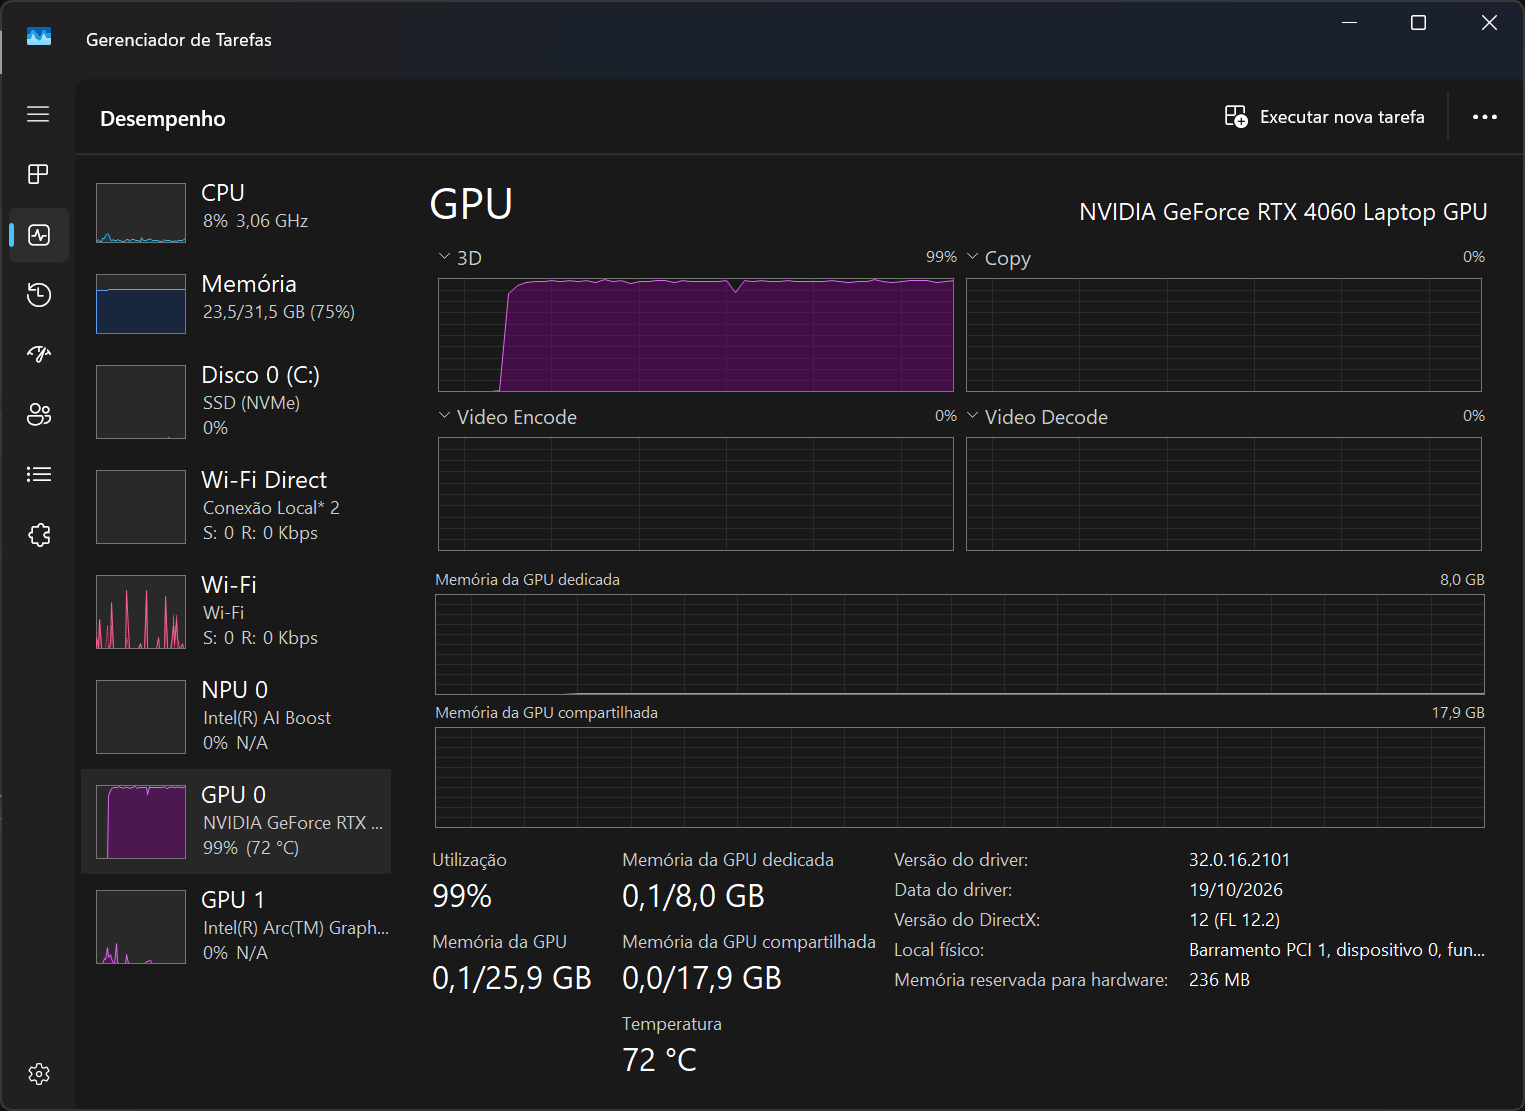
\includegraphics[width=\textwidth]{gpu-nvidia.png}\caption{GPU 0: NVIDIA GeForce RTX 4060 Laptop (3D a 99\%)}\end{subfigure}\\[0.5em]
\begin{subfigure}{0.78\textwidth}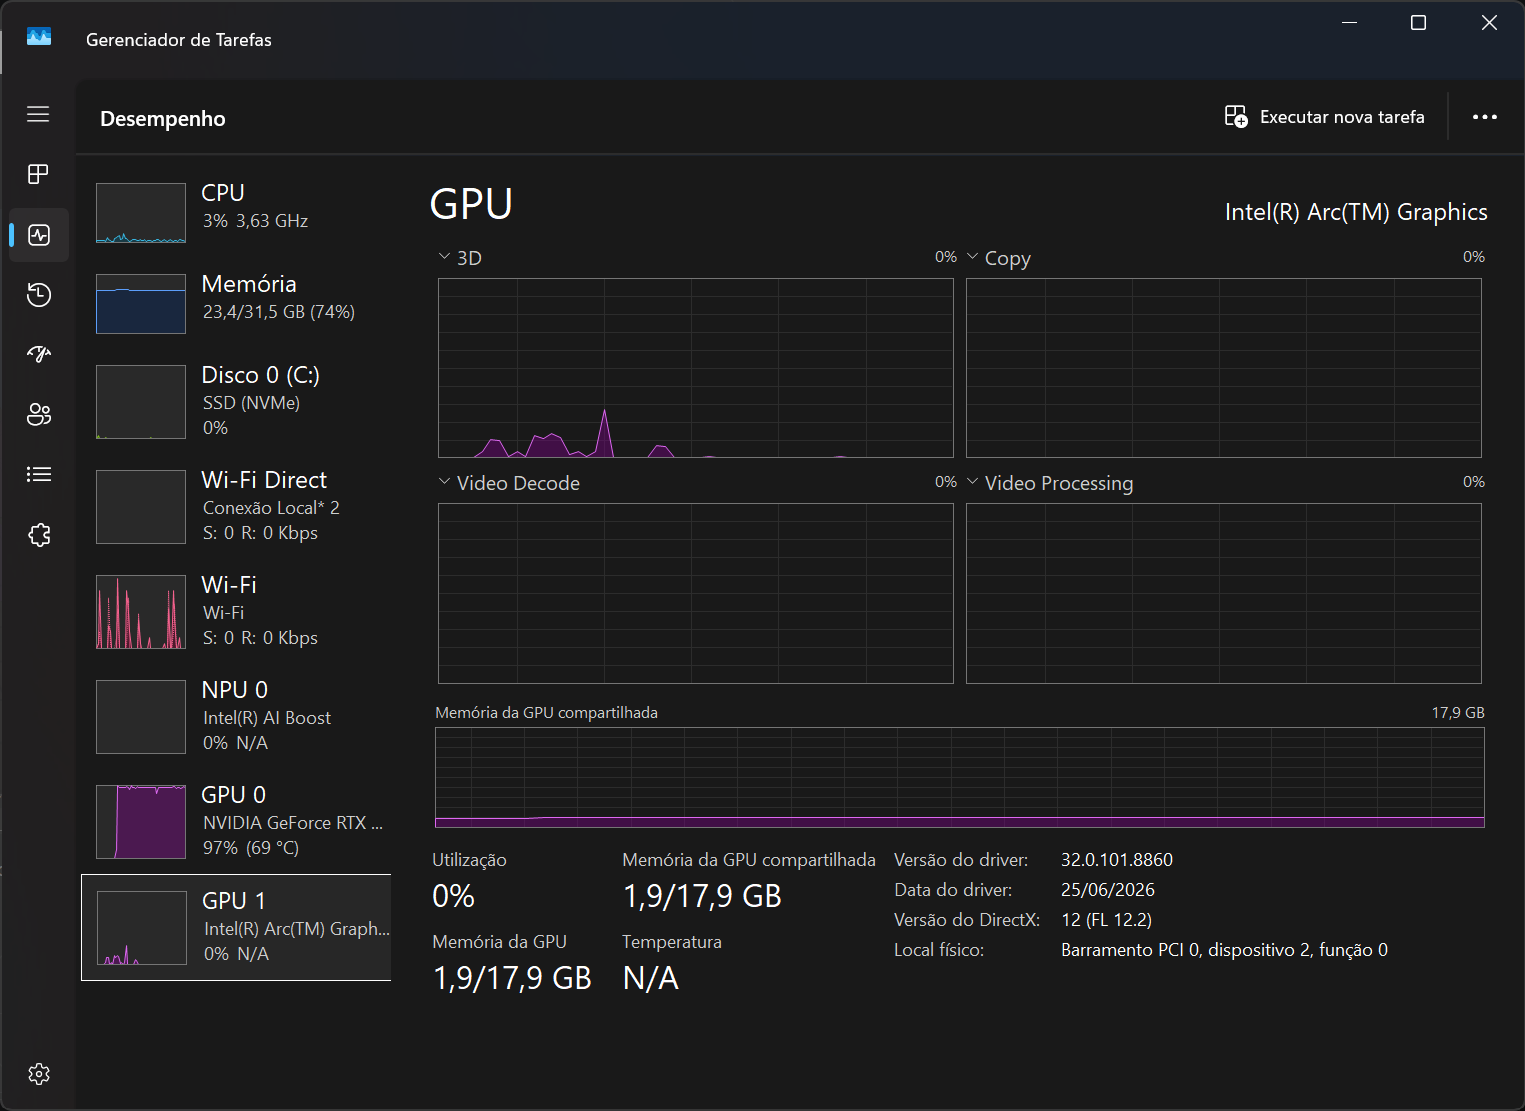
\includegraphics[width=\textwidth]{gpu-intel.png}\caption{GPU 1: Intel Arc Graphics (3D a 0\%)}\end{subfigure}
\caption{Gerenciador de Tarefas do Windows aos 50~s de uma medição na configuração F com
$T=576$ (84,8 milhões de triângulos), com as duas GPUs acompanhadas separadamente.}
\label{fig:taskmgr}
\end{figure}

A Figura~\ref{fig:painel_tm} mostra o painel da própria aplicação no mesmo instante (50,5~s da
medição). As medições internas concordam com o Gerenciador de Tarefas: motor 3D do processo a
95\% na NVIDIA e 0\% na Intel, NVML com 100\% de utilização, 60~W (o limite de potência) e clock
reduzido a 2\,280~MHz, CPU do processo a 0,8\%. A decomposição do quadro mostra o gargalo
diretamente: dos 17,43~ms do quadro, a GPU trabalha 17,40~ms, enquanto a thread principal
executa só 0,16~ms de CPU. O tempo de emissão (17,25~ms) é quase todo \emph{espera} dentro do
\emph{driver}, que bloqueia a thread quando a fila de comandos para a GPU está cheia; por isso a
thread aparece com apenas 3\% de uso apesar de passar o quadro inteiro ``dentro'' da emissão.

\begin{figure}[H]
\centering
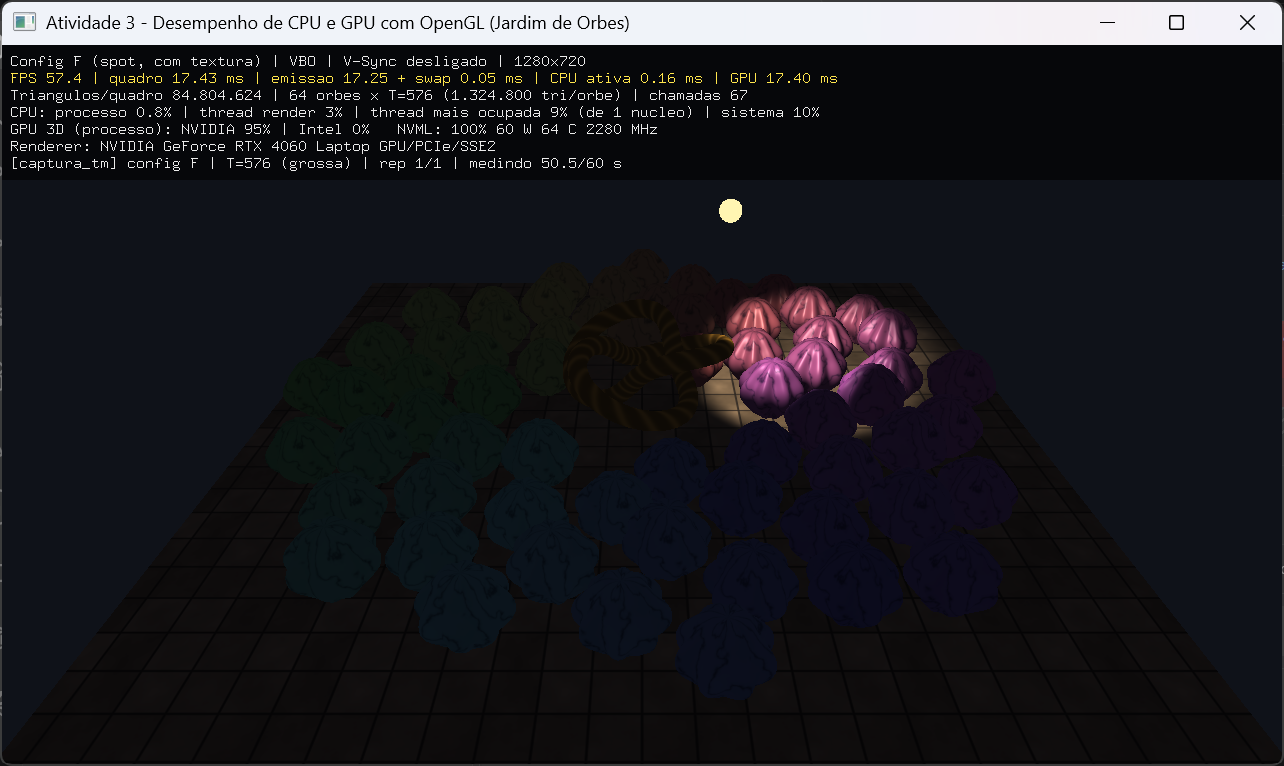
\includegraphics[width=0.9\textwidth]{painel_captura_tm.png}
\caption{Janela da aplicação aos 50,5~s da mesma medição (configuração F, $T=576$), com o painel
de medições em tempo real.}
\label{fig:painel_tm}
\end{figure}

% ===========================================================================
\section{Descrição da cena e da estratégia de polígonos}
% ===========================================================================

\subsection{A cena ``Jardim de Orbes''}

A cena, de autoria própria, é composta por (Figura~\ref{fig:cenas}):
\begin{itemize}
  \item um \textbf{piso} de ladrilhos ($48\times48$ quadrados, 4\,608 triângulos);
  \item um \textbf{nó toroidal} dourado do tipo $(2,3)$ no centro, com seção circular
        ($256\times24$ quadriláteros, 12\,288 triângulos), que \textbf{gira continuamente} em dois
        eixos e flutua;
  \item $N$ \textbf{orbes} de mármore (esferas com relevo em gomos) dispostos em espiral
        filotáxica --- o padrão das sementes de girassol, com ângulo de ouro
        $\pi(3-\sqrt5)\approx137{,}5^\circ$ entre orbes consecutivos e raio $\propto\sqrt{i}$ ---
        que giram em carrossel em torno do nó, cada um girando sobre si e oscilando na vertical;
  \item uma \textbf{lâmpada}, pequena esfera emissiva que marca a posição da fonte de luz
        (528 triângulos), desenhada em todas as configurações.
\end{itemize}
A câmera é fixa, a janela tem sempre $1280\times720$ pixels e a animação depende só do tempo
real, de modo que todas as configurações mostram a mesma cena. A luz omnidirecional orbita o
centro a 4,5 unidades de altura; o \emph{spot} fica a 7 unidades de altura e varre o piso com
seu cone.

\begin{figure}[H]
\centering
\begin{subfigure}{0.49\textwidth}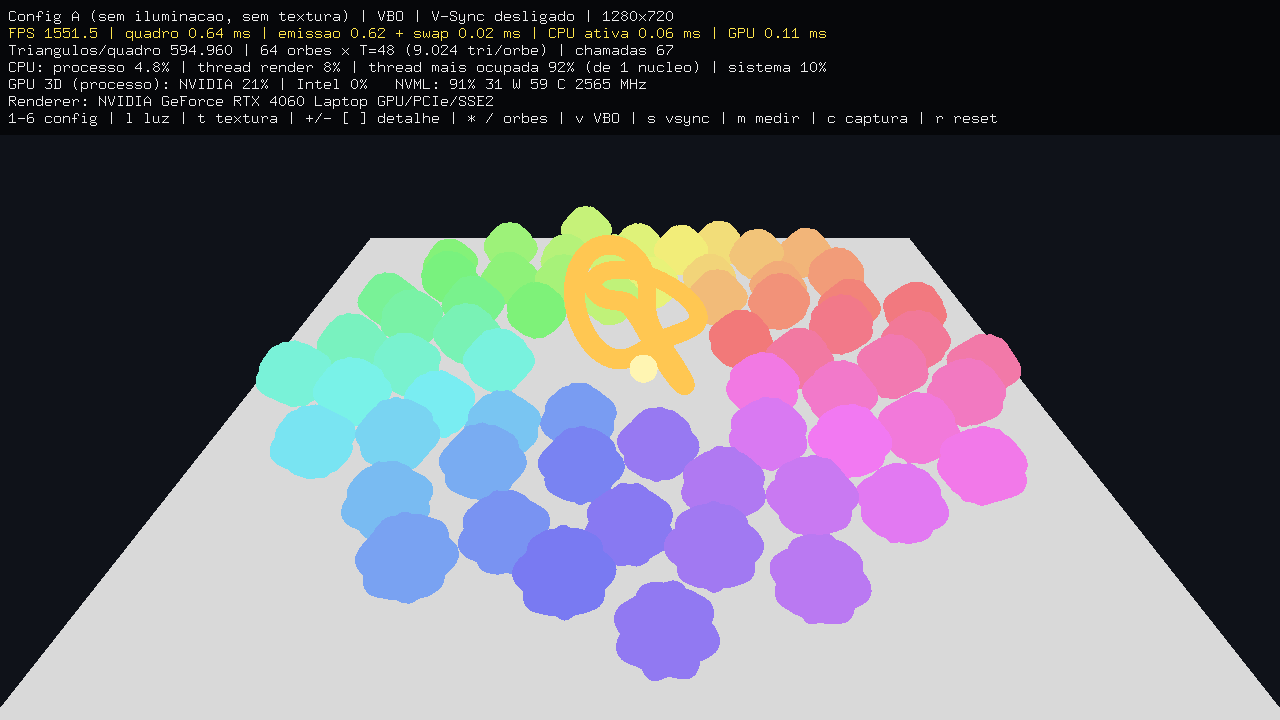
\includegraphics[width=\textwidth]{cena_A.png}\caption{A: sem luz, sem textura}\end{subfigure}
\begin{subfigure}{0.49\textwidth}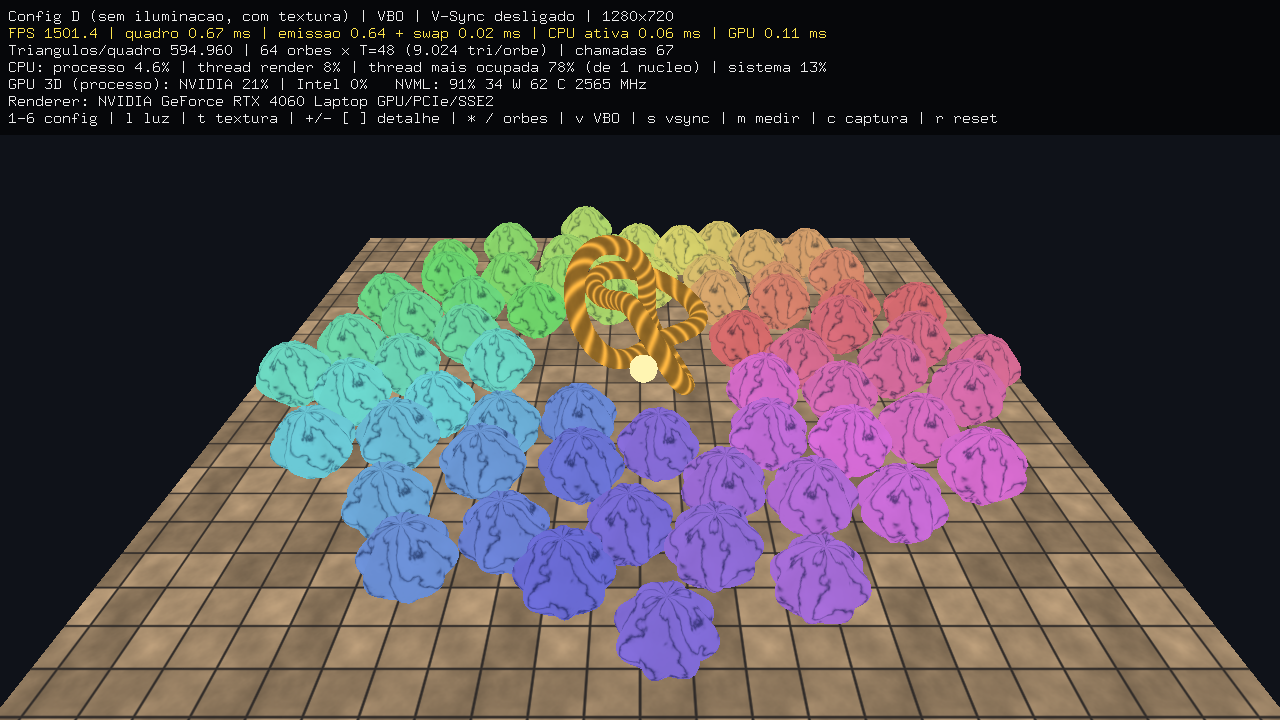
\includegraphics[width=\textwidth]{cena_D.png}\caption{D: sem luz, com textura}\end{subfigure}\\[0.3em]
\begin{subfigure}{0.49\textwidth}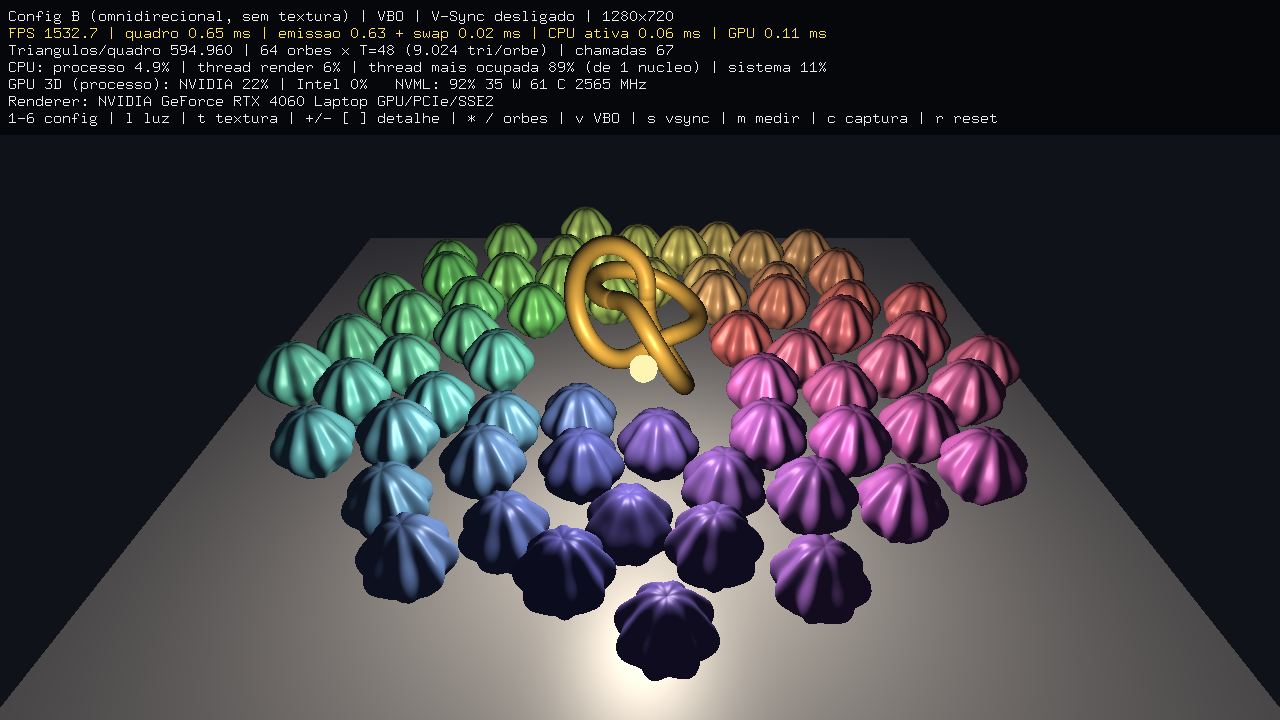
\includegraphics[width=\textwidth]{cena_B.png}\caption{B: omnidirecional, sem textura}\end{subfigure}
\begin{subfigure}{0.49\textwidth}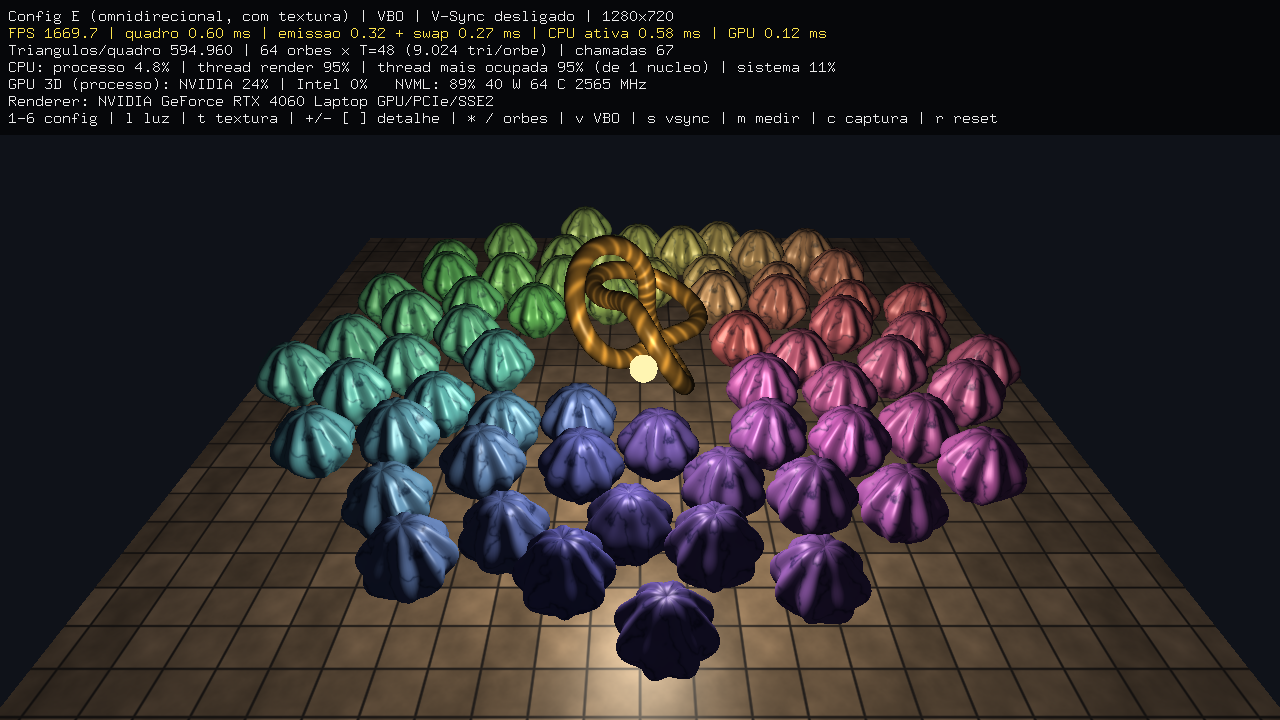
\includegraphics[width=\textwidth]{cena_E.png}\caption{E: omnidirecional, com textura}\end{subfigure}\\[0.3em]
\begin{subfigure}{0.49\textwidth}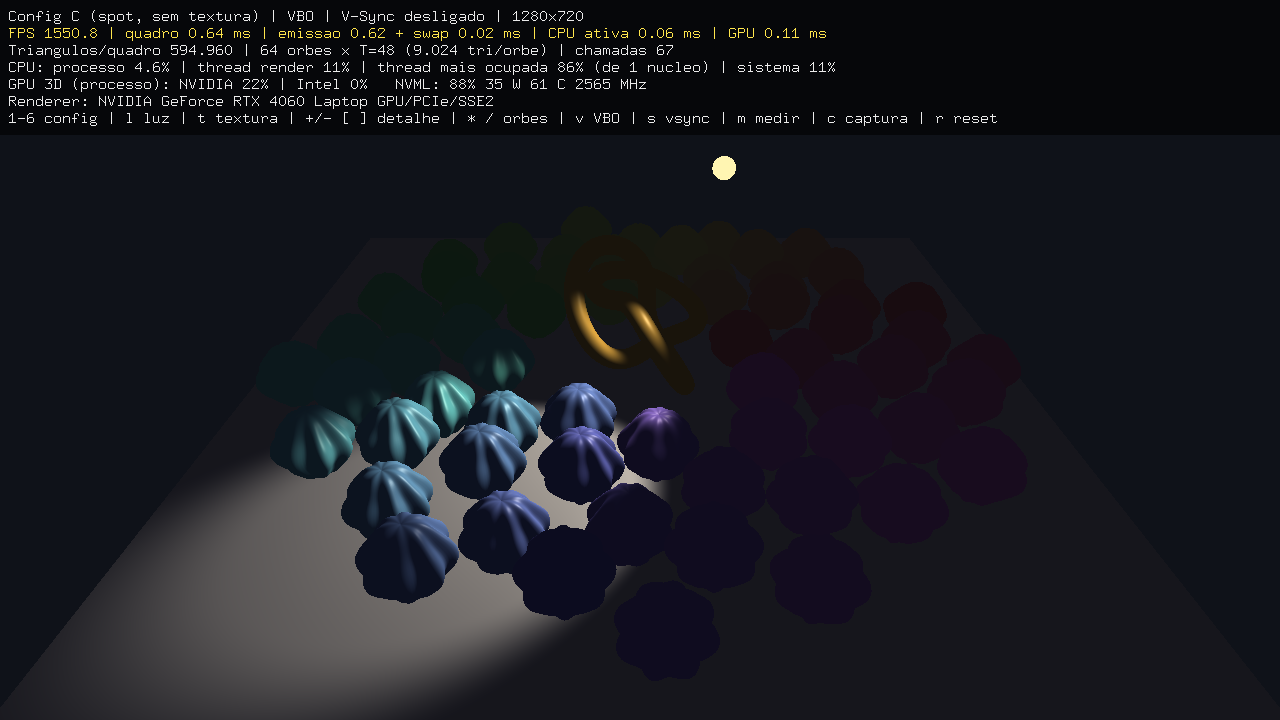
\includegraphics[width=\textwidth]{cena_C.png}\caption{C: spot, sem textura}\end{subfigure}
\begin{subfigure}{0.49\textwidth}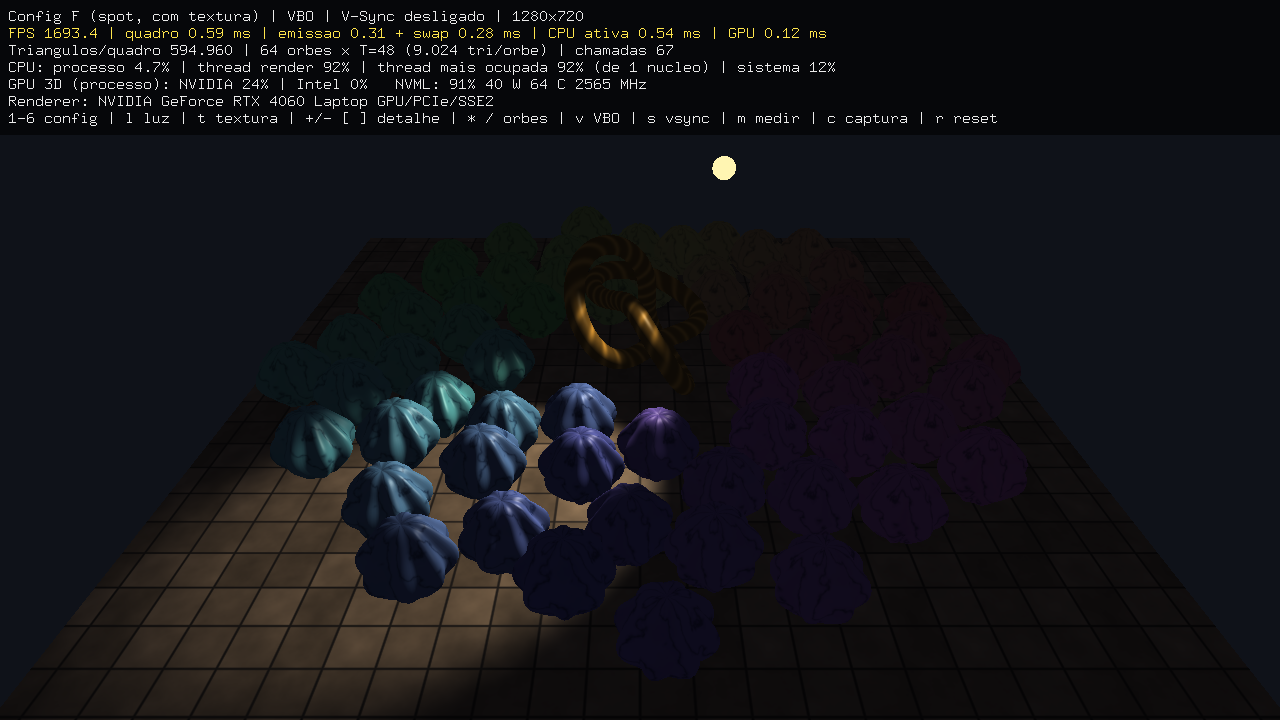
\includegraphics[width=\textwidth]{cena_F.png}\caption{F: spot, com textura}\end{subfigure}
\caption{As seis configurações experimentais no mesmo instante da animação ($T=48$, $N=64$,
594\,960 triângulos por quadro). O painel superior mostra o FPS e as medições em tempo real.}
\label{fig:cenas}
\end{figure}

A Figura~\ref{fig:cenas} confirma que a iluminação produz resultado verificável: em A e D os
objetos têm cor uniforme (sem sombreamento); em B e E a luz omnidirecional (esfera clara à frente
do nó) produz sombreamento difuso, reflexos especulares e atenuação com a distância; em C e F
apenas a região dentro do cone do \emph{spot} é iluminada, com borda suave. As texturas (D, E, F)
mostram os ladrilhos do piso, os veios de mármore dos orbes e as faixas trançadas do nó.

\subsection{Estratégia de aumento dos polígonos}

A carga geométrica é controlada por dois parâmetros independentes:
\begin{itemize}
  \item $T$, o \textbf{nível de detalhe} de cada orbe: o orbe é uma superfície paramétrica com
        $T$ faixas de latitude e $2T$ de longitude. Aumentar $T$ aumenta os triângulos de cada
        objeto sem mudar o número de objetos, de chamadas de desenho ou de pixels cobertos;
  \item $N$, o \textbf{número de orbes}: aumentar $N$ aumenta os triângulos e também o número de
        chamadas de desenho (uma por orbe). Para manter a área ocupada na tela aproximadamente
        constante, o raio de cada orbe diminui com $\sqrt{N}$.
\end{itemize}
O experimento principal (E1) varia $T$ com $N=64$ fixo, isolando o efeito da quantidade de
polígonos. O experimento E3 varia $N$ com $T=8$, para observar o efeito do número de objetos.

\begin{figure}[H]
\centering
\begin{subfigure}{0.49\textwidth}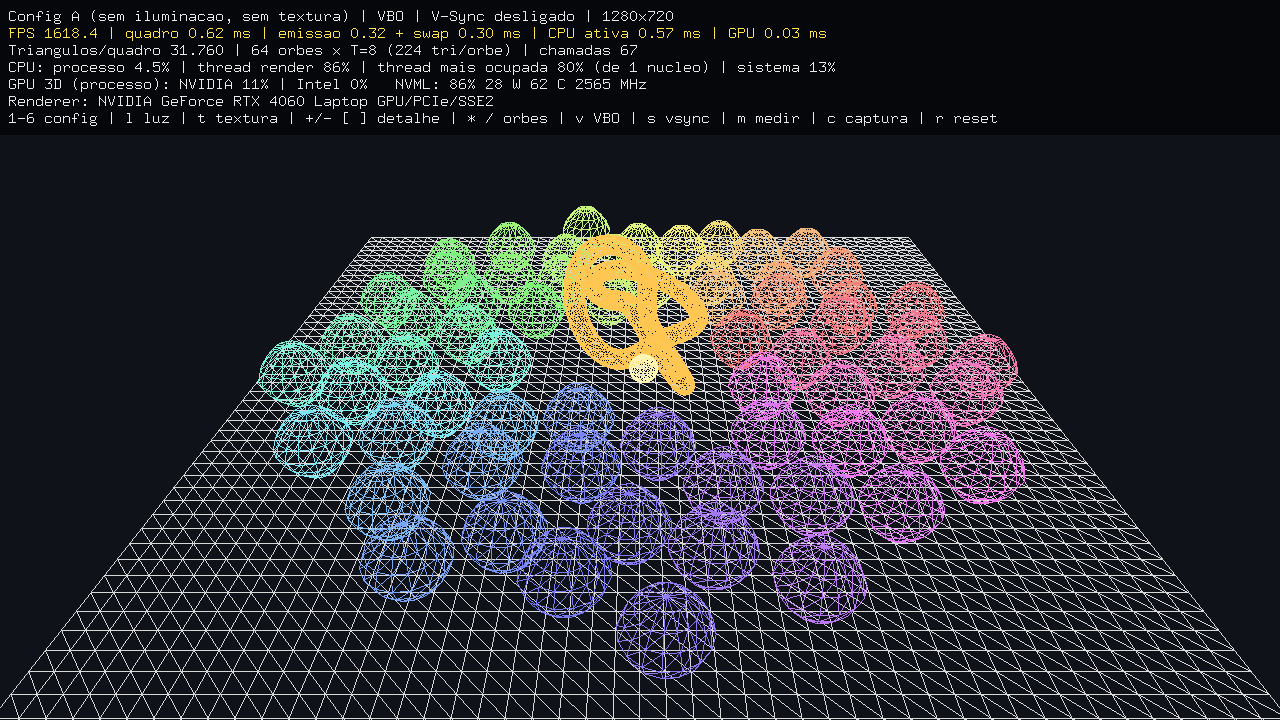
\includegraphics[width=\textwidth]{aramado_T8.png}\caption{$T=8$: 224 triângulos por orbe}\end{subfigure}
\begin{subfigure}{0.49\textwidth}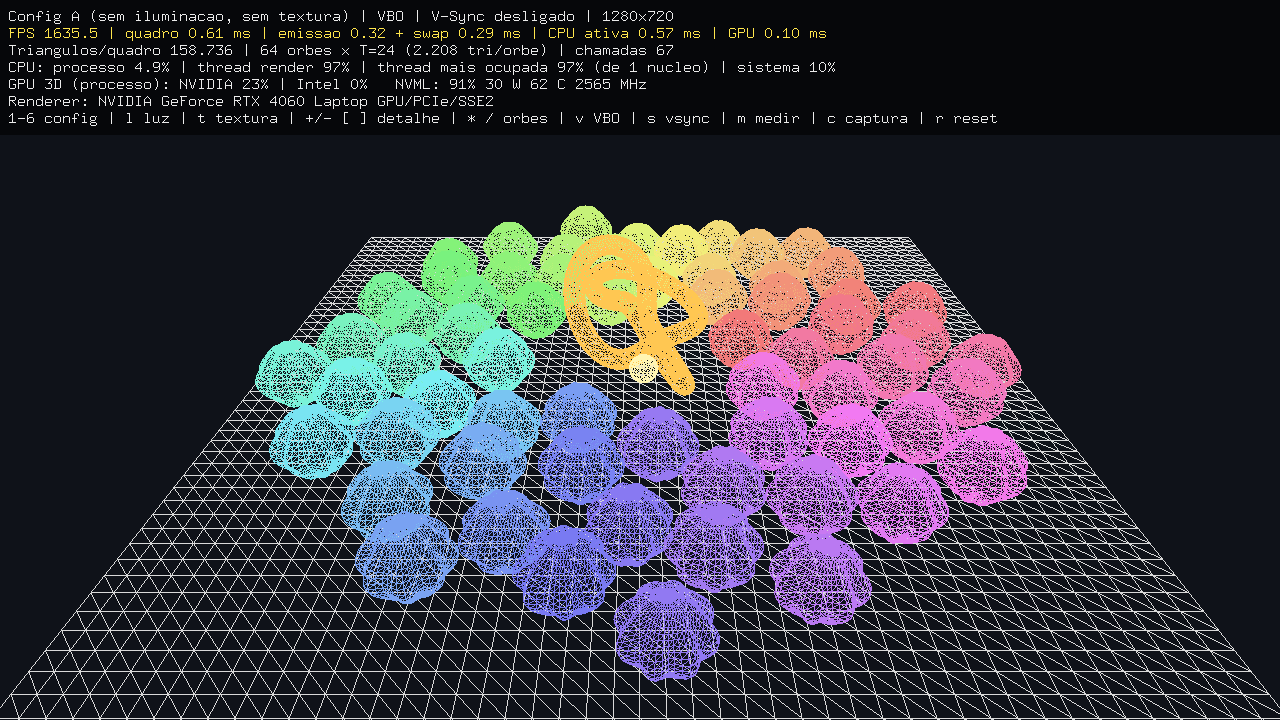
\includegraphics[width=\textwidth]{aramado_T24.png}\caption{$T=24$: 2\,208 triângulos por orbe}\end{subfigure}
\caption{Desenho em arame (tecla \code{w}) mostrando o aumento do detalhe $T$ dos orbes.}
\label{fig:aramado}
\end{figure}

\subsection{Critério de contagem dos polígonos}

\begin{itemize}
  \item Toda a geometria da cena é formada \textbf{exclusivamente por triângulos} indexados
        (\code{GL_TRIANGLES}). Não há quadriláteros, leques ou faixas: cada quadrilátero de uma
        superfície paramétrica é gerado como 2 triângulos e já contado assim. Portanto,
        ``polígonos'' neste relatório significa \textbf{triângulos}.
  \item A contagem é \textbf{exata}: cada malha tem \code{indices.size()/3} triângulos, e o total
        por quadro é a soma sobre todos os objetos desenhados:
        \begin{equation}
          \text{triângulos/quadro} = \underbrace{4\,608 + 12\,288 + 528}_{\text{cenário fixo} = 17\,424}
          + N \cdot 4T(T-1).
        \end{equation}
        O orbe tem $2T$ colunas e $T$ faixas; as faixas dos dois polos colapsam num ponto e nelas
        só é gerado o triângulo não degenerado de cada quadrilátero, daí
        $2\cdot 2T\cdot T - 2\cdot 2T = 4T(T-1)$ triângulos.
  \item Contam-se os triângulos \textbf{submetidos} ao \emph{pipeline} a cada quadro, antes do
        recorte e do \emph{back-face culling} (habilitado). Como a câmera é fixa e todos os
        objetos ficam dentro do campo de visão, praticamente nada é recortado; o
        \emph{culling} descarta, na GPU, cerca de metade dos triângulos (as faces de trás), mas
        só depois de os vértices terem sido processados.
  \item O painel de texto e seu fundo (2 triângulos) são interface e não são contados.
  \item O valor é mostrado no painel da janela e gravado em cada linha dos arquivos CSV.
\end{itemize}

% ===========================================================================
\section{Metodologia de coleta e medição}
% ===========================================================================

\subsection{Cálculo do FPS e dos tempos}

A cada quadro, a aplicação registra quatro instantes e grandezas (\code{main.cpp}):
\begin{itemize}
  \item \textbf{tempo de emissão}: tempo de relógio entre o início do quadro e o fim da emissão dos
        comandos OpenGL (antes de \code{glutSwapBuffers}). Pode incluir esperas dentro do
        \emph{driver};
  \item \textbf{tempo de \emph{swap}}: tempo bloqueado em \code{glutSwapBuffers};
  \item \textbf{CPU ativa}: ciclos de CPU realmente executados pela thread principal no quadro
        (\code{QueryThreadCycleTime}, convertidos em ms pela frequência do contador de ciclos,
        calibrada na inicialização). Ao contrário dos dois tempos anteriores, \emph{não} inclui o
        tempo em que a thread ficou bloqueada esperando;
  \item \textbf{tempo de GPU}: medido pela própria GPU com consultas \code{GL_TIME_ELAPSED} em
        torno de todos os comandos do quadro. Os resultados são lidos sem bloquear, alguns
        quadros depois (só são consultadas as consultas com pelo menos 3 quadros de idade, pois
        perguntar por uma consulta recente força o \emph{driver} a esvaziar a fila e alteraria a
        própria medição).
\end{itemize}
Numa janela de medição, $\text{FPS médio} = n/\Delta t$, com $n$ o número de quadros concluídos
(contados após o \emph{swap}) e $\Delta t$ o tempo entre o início da janela e o fim do último
quadro; o tempo médio por quadro é $1000/\text{FPS}$. As demais grandezas são médias por quadro.

\subsection{Utilização de CPU, GPU e memória}

Uma thread auxiliar (fora da thread de renderização) coleta amostras a cada 500~ms
(\code{monitor.cpp}):
\begin{itemize}
  \item \textbf{CPU do processo}: \code{GetProcessTimes}, em \% da CPU inteira (22 threads
        lógicas), como no Gerenciador de Tarefas;
  \item \textbf{thread principal} e \textbf{thread mais ocupada do processo}: tempo de CPU de cada
        thread (\code{Toolhelp32} + \code{GetThreadTimes}), em \% de \emph{um} núcleo. A thread mais
        ocupada pode ser uma thread interna do \emph{driver} OpenGL;
  \item \textbf{GPU}: contadores PDH \code{\GPU Engine(*)\Utilization Percentage} (motor 3D do
        processo em cada GPU) e \code{\GPU Process Memory(*)} (memória de vídeo do processo);
  \item \textbf{NVML}: utilização, controlador de memória, potência, temperatura, clocks e motivos
        de redução de clock (por exemplo, ``limite de potência'') da GPU NVIDIA;
  \item \textbf{RAM}: \emph{working set} do processo e carga de memória do sistema.
\end{itemize}

\subsection{Protocolo experimental}

O protocolo foi automatizado (\code{benchmark.cpp}) para garantir procedimentos idênticos em todos
os pontos:
\begin{enumerate}
  \item janela fixa de $1280\times720$ pixels (a aplicação é \emph{DPI-aware}, então são pixels
        reais), câmera, animação e cena idênticas; V-Sync desligado pela aplicação e o painel de
        controle da NVIDIA em ``usar configuração do aplicativo''; sem limitador de FPS;
  \item para cada configuração (A a F), varredura \textbf{grossa} de uma lista crescente de valores
        de $T$, começando por uma carga leve, que serve de referência;
  \item em cada ponto: aplica a carga, \textbf{estabiliza 2~s} (descartados), \textbf{mede 10~s};
        repete \textbf{3 vezes} (cada repetição com nova estabilização) e calcula a média e o
        desvio-padrão amostral do FPS e a média das demais grandezas;
  \item o critério de ``abaixo de 60'' é o \textbf{FPS médio das 3 repetições};
  \item ao encontrar o primeiro ponto com FPS médio $<60$, faz \textbf{refino por bisseção} em $T$
        entre o último ponto $\geq 60$ e o primeiro $<60$, até que as cargas difiram em no máximo
        5\% de triângulos;
  \item continua a varredura grossa até o FPS cair abaixo de um limiar de parada (35 ou 30 FPS),
        para mostrar a tendência após o limite;
  \item registra, para cada configuração, a \textbf{menor quantidade testada} de triângulos com FPS
        médio $<60$ e a situação do teste.
\end{enumerate}
Os testes foram executados em sequência pelo \emph{script} de experimentos, com o notebook ligado à tomada e sem outros aplicativos abertos além dos processos do sistema.
Todos os valores brutos (cada repetição) e agregados (cada ponto) estão nos arquivos CSV em
\code{resultados/dados}.

\subsection{Experimentos realizados}

\begin{table}[H]
\centering
\caption{Experimentos. Em todos: janela $1280\times720$, V-Sync desligado, 3 repetições de 10~s.}
\label{tab:experimentos}
\small
\begin{tabularx}{\textwidth}{l l l L c}
\toprule
Exp. & GPU & Envio & Variável (valores da varredura grossa) & Config. \\
\midrule
E1 & RTX 4060 & VBO & $T$ = 16, 64, 128, 192, \dots, 512, 640, 768 ($N=64$) & A--F \\
E2 & RTX 4060 & imediato & $T$ = 8, 16, 24, 32, 48, 64 ($N=64$) & A--F \\
E3 & RTX 4060 & VBO & $N$ = 64, 256, 1\,024, \dots, 65\,536 ($T=8$) & A, F \\
E4 & Intel Arc & VBO & $T$ = 16, 64, 128, 192, 256, 320 ($N=64$) & A--F \\
\bottomrule
\end{tabularx}
\end{table}
O E1 é o experimento principal exigido. E2, E3 e E4 são complementares: mudam \emph{onde} está
a carga (CPU \emph{versus} GPU) para testar as hipóteses de gargalo levantadas no E1.

% ===========================================================================
\section{Implementação das funcionalidades gráficas}
% ===========================================================================

\subsection{Organização do código}

\begin{table}[H]
\centering
\caption{Arquivos do projeto (código completo no Anexo).}
\label{tab:arquivos}
\small
\begin{tabularx}{\textwidth}{l L}
\toprule
Arquivo & Responsabilidade \\
\midrule
\code{gl_ext.h/.cpp} & carregamento das funções OpenGL $>$ 1.1 (\emph{shaders}, VBO, consultas, V-Sync) \\
\code{malha.h/.cpp} & malhas de triângulos: geração do orbe, do nó e do piso; VBO e modo imediato \\
\code{texturas.h/.cpp} & texturas procedurais ($1024^2$, ruído periódico, \emph{mipmaps}, anisotropia) \\
\code{shaders.h/.cpp} & fonte GLSL e compilação das 6 variantes (iluminação $\times$ textura) \\
\code{cena.h/.cpp} & cena, animação, luzes, configurações A--F e contagem de triângulos \\
\code{monitor.h/.cpp} & monitoramento de CPU, GPU, memória, potência (PDH, DXGI, NVML) \\
\code{benchmark.h/.cpp} & medição dos quadros e protocolo automático com CSV \\
\code{main.cpp} & FreeGLUT, laço de quadros, painel, teclado, capturas, linha de comando \\
\code{tools/graficos.py} & gráficos e tabelas do relatório a partir dos CSV \\
\bottomrule
\end{tabularx}
\end{table}

\subsection{Geometria}

As malhas são geradas proceduralmente por uma função genérica que amostra uma superfície
paramétrica $\mathbf{P}(u,v)$ numa grade e calcula a normal de cada vértice como
$\partial\mathbf{P}/\partial u\times\partial\mathbf{P}/\partial v$ por diferenças centrais, o que
dá normais suaves e contínuas nas emendas. O orbe usa
$r(\theta,\phi)=1+0{,}1\sin(8\theta)\sin^2\phi+0{,}05\sin(5\phi)$ (gomos); o nó toroidal $(2,3)$ usa
o referencial de Frenet da curva central. Cada vértice tem posição, normal e coordenada de textura
(32 bytes). Os triângulos são orientados no sentido anti-horário visto de fora, permitindo o
\emph{back-face culling}.

A mesma malha pode ser enviada de duas formas (tecla \code{v}): por \textbf{VBO} (vértices e índices
na memória da GPU; um \code{glDrawElements} por objeto) ou em \textbf{modo imediato}
(\code{glBegin}/\code{glEnd} com \code{glTexCoord2f}, \code{glNormal3f} e \code{glVertex3f} para cada
vértice de cada triângulo, a cada quadro). Ao mudar $T$, a malha do orbe é recriada e reenviada
para a GPU; os $N$ orbes compartilham a mesma malha e diferem apenas na matriz de modelagem e na
cor.

\subsection{Iluminação e texturas com GLSL}

A iluminação é calculada por fragmento num \emph{fragment shader} GLSL 1.20, que implementa a
Equação~\eqref{eq:blinn}. O \emph{vertex shader} transforma posição e normal para coordenadas do
observador. Uma única fonte de \emph{shader} é compilada em \textbf{seis variantes}, uma para cada
combinação de iluminação (\code{ILUMINACAO} = 0, 1 ou 2) e textura (\code{TEXTURA} = 0 ou 1),
selecionadas por \code{\#define}. Assim cada configuração executa somente o código de que precisa:
a configuração A não calcula iluminação nem lê texturas, e não há desvios condicionais em tempo de
execução que pudessem mascarar o custo de cada recurso. As posições da luz e a direção do \emph{spot}
são animadas na CPU e enviadas como \emph{uniforms} em coordenadas do observador.

As três texturas ($1024\times1024$ RGBA, 16~MB no total com \emph{mipmaps}) são geradas por código
na inicialização, com ruído de valor periódico (sem emendas ao repetir): ladrilhos de arenito
(piso), mármore com veios (orbes) e faixas trançadas (nó). Usam filtragem trilinear e anisotrópica
8x. Sem textura, a cor é a do material; com textura, a cor do material é multiplicada pela cor
amostrada.

\subsection{Comandos de teclado e reprodução dos experimentos}

\begin{table}[H]
\centering
\caption{Comandos de teclado da aplicação.}
\label{tab:teclas}
\small
\begin{tabularx}{\textwidth}{l L}
\toprule
Tecla & Ação \\
\midrule
\code{1} a \code{6} & seleciona a configuração A a F \\
\code{l} & alterna a iluminação: nenhuma $\to$ omnidirecional $\to$ spot \\
\code{t} & liga/desliga as texturas \\
\code{+} / \code{-} & aumenta/diminui o detalhe $T$ dos orbes (passo 4 abaixo de 64, 16 acima) \\
\code{]} / \code{[} & ajuste fino de $T$ ($\pm1$) \\
\code{*} / \code{/} & dobra/reduz à metade o número de orbes $N$ \\
\code{v} & alterna VBO e modo imediato \\
\code{s} & liga/desliga o V-Sync \\
\code{w} & desenho em arame \\
\code{p} & pausa/retoma a animação \\
\code{h} & mostra/oculta o painel \\
\code{c} & salva captura de tela em \code{resultados/capturas} \\
\code{m} & mede o ponto atual (3 $\times$ 10~s) e grava em \code{resultados/dados/manual_*.csv} \\
\code{r} ou \code{Home} & restaura a configuração inicial (A, $T=32$, $N=64$, VBO, V-Sync desligado) \\
\code{ESC} ou \code{q} & encerra \\
\bottomrule
\end{tabularx}
\end{table}

Para reproduzir os experimentos: (1) compilar com \code{build.bat}; (2) executar
\code{executar_experimentos.bat} na raiz do projeto, que gera as capturas, executa E1--E4
(cerca de 2h30) e os gráficos; ou (3) executar manualmente, por exemplo,
\code{build\Release\desempenho_gl.exe --benchmark --rotulo teste --configs C --valores 256,512}.
No modo interativo, qualquer ponto pode ser medido com a tecla \code{m}, sem recompilar.

% ===========================================================================
\section{Resultados do experimento principal (E1)}
% ===========================================================================

\subsection{Execução da coleta}

Os quatro experimentos somaram 90 pontos de carga $\times$ configuração no E1, 60 no E2, 24 no
E3 e 60 no E4, cada um com 3 repetições de 10~s após 2~s de estabilização. Durante o E1, na
configuração F, a janela da aplicação foi minimizada por engano; minimizada, a janela deixa de
receber eventos de desenho do FreeGLUT e a medição ficou parada por cerca de uma hora. A
repetição afetada foi descartada e a configuração F foi \textbf{medida novamente do início}, em
arquivo próprio (\code{e1_vbo_T_F_*.csv}), que substitui a F incompleta. Para que isso não se
repita, o protocolo passou a descartar e reiniciar automaticamente qualquer repetição em que o
intervalo entre dois quadros exceda 2~s; nenhuma ocorrência foi registrada no restante da coleta.
As configurações A a E não foram afetadas. A comparação entre a F original e a nova, nos pontos
comuns, mostra diferenças de 0,1 a 0,3\% para $T$ entre 128 e 256 (região limitada pela GPU) e de
até 10\% para $T=16$, região limitada pela CPU, em que o FPS passa de 1\,500 e é mais sensível a
variações do clock e do escalonamento da CPU (Seção~\ref{sec:gargalos}).

\subsection{FPS em função da quantidade de triângulos}

As Figuras~\ref{fig:g1} a \ref{fig:g4} mostram o FPS médio em função dos triângulos por
quadro, com a linha de referência de 60~FPS. Os eixos são logarítmicos porque a carga varia de
$7{,}9\times10^4$ a $1{,}5\times10^8$ triângulos e o FPS de $\approx$1\,800 a $\approx$32.

\begin{figure}[H]
\centering
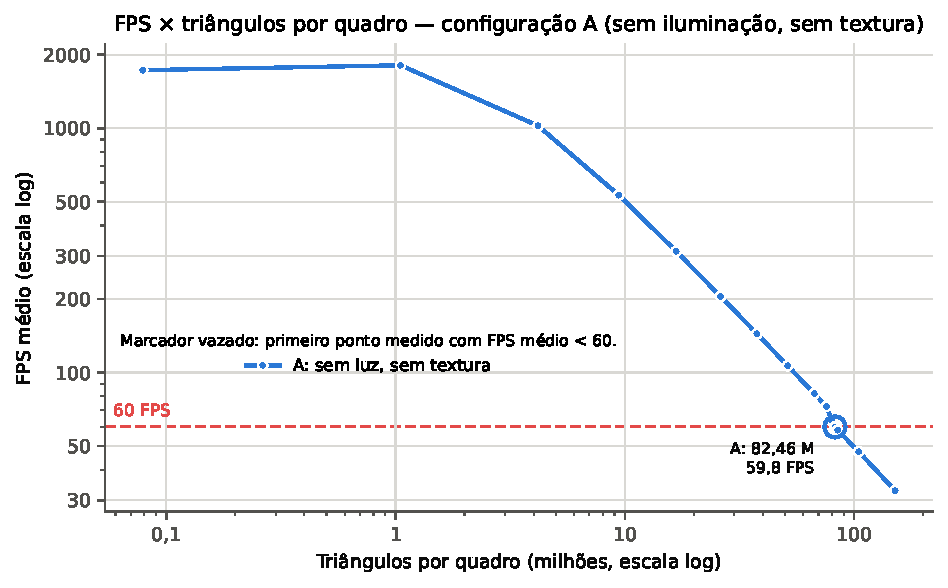
\includegraphics[width=0.86\textwidth]{g1_fps_A.pdf}
\caption{FPS médio $\times$ triângulos por quadro na configuração A (E1). O marcador vazado
indica a menor carga testada com FPS médio abaixo de 60.}
\label{fig:g1}
\end{figure}

\begin{figure}[H]
\centering
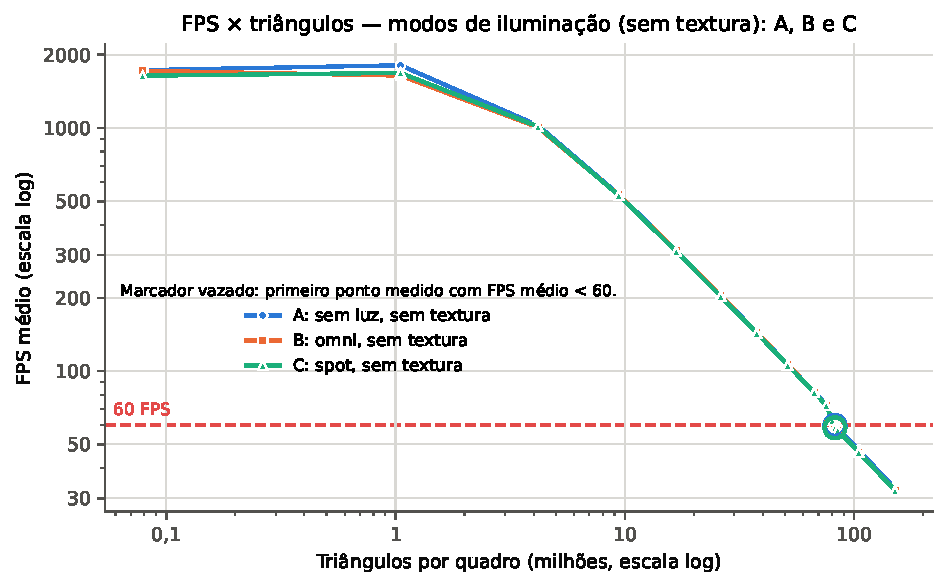
\includegraphics[width=0.86\textwidth]{g2_fps_iluminacao.pdf}
\caption{FPS médio $\times$ triângulos para os três modos de iluminação sem textura (A, B e C).}
\label{fig:g2}
\end{figure}

\begin{figure}[H]
\centering
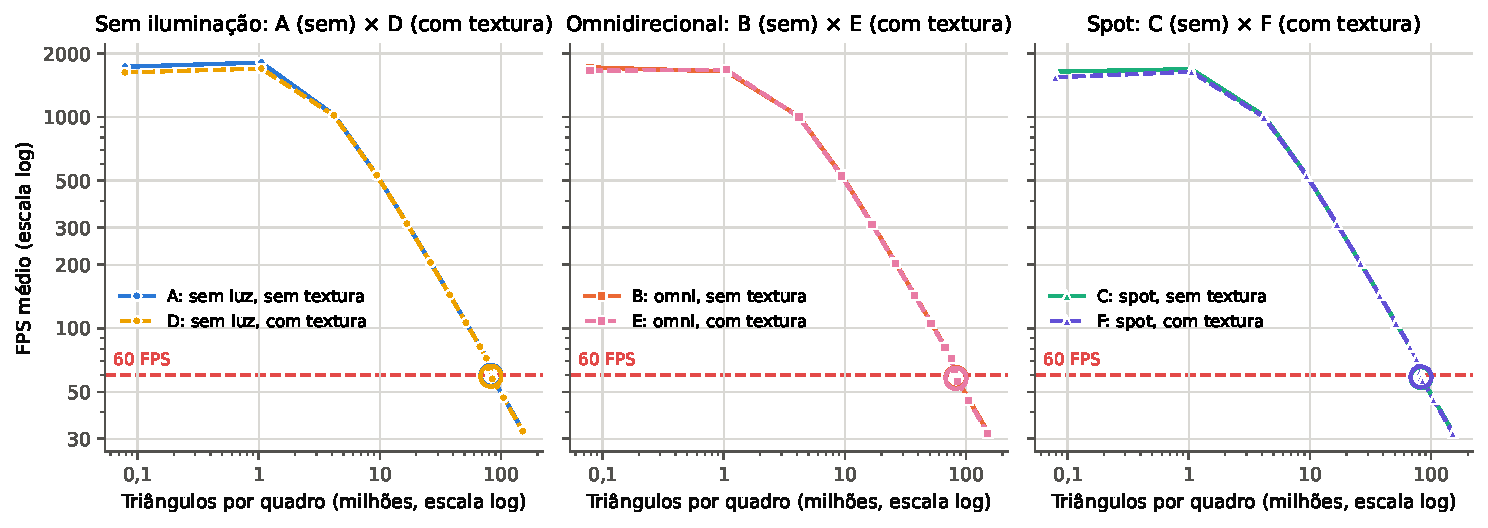
\includegraphics[width=\textwidth]{g3_fps_textura.pdf}
\caption{Efeito das texturas: cada painel compara a mesma iluminação sem e com textura
(A$\times$D, B$\times$E, C$\times$F).}
\label{fig:g3}
\end{figure}

\begin{figure}[H]
\centering
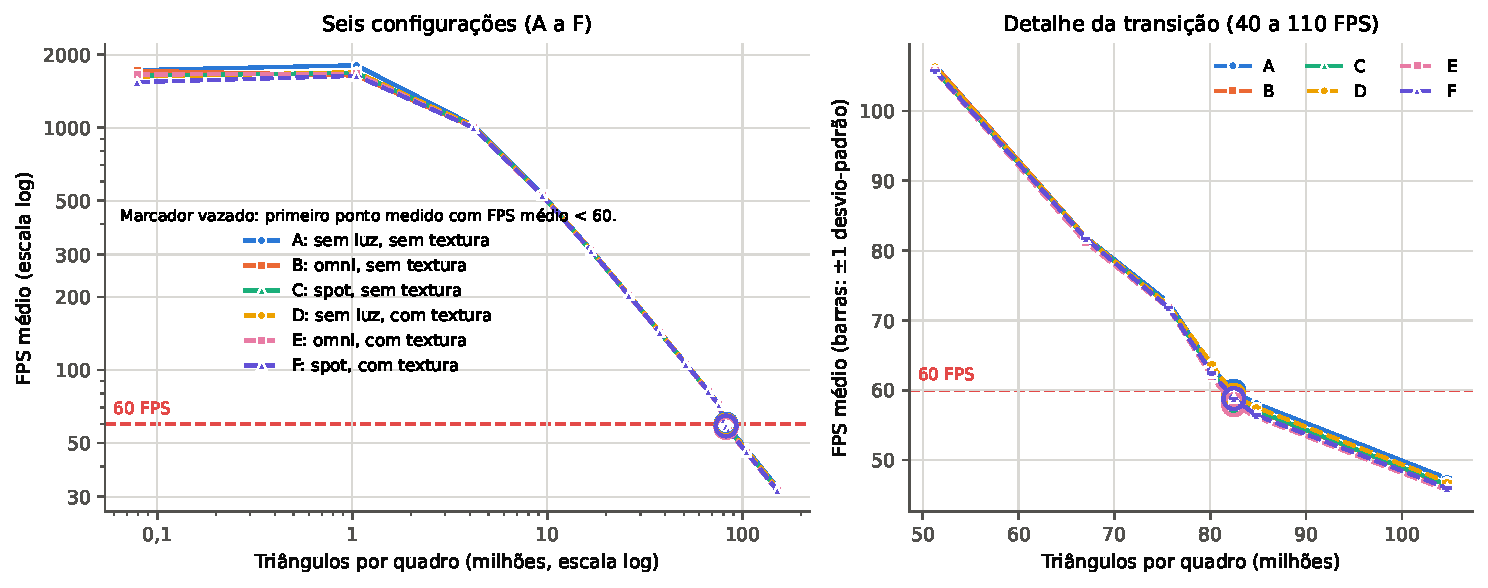
\includegraphics[width=\textwidth]{g4_fps_seis_configuracoes.pdf}
\caption{As seis configurações. À direita, a região próxima de 60~FPS em escala linear, com
barras de $\pm1$ desvio-padrão das 3 repetições (menores que os marcadores).}
\label{fig:g4}
\end{figure}

As curvas têm três trechos. Até $\approx$1 milhão de triângulos o FPS é praticamente constante
($\approx$1\,550--1\,800~FPS): a quantidade de geometria ainda não é o que limita o quadro. A
partir de $\approx$4 milhões o FPS passa a cair na \textbf{proporção inversa} dos triângulos (reta
de inclinação $-1$ no gráfico log-log): dobrar os triângulos reduz o FPS à metade. Perto de 80
milhões há um ``joelho'' (detalhe da Figura~\ref{fig:g4}): entre 75,6 e 80,2 milhões de
triângulos (+6\%) o FPS cai 13\%, mais que o proporcional; a causa é investigada na
Seção~\ref{sec:gargalos}.

As seis curvas são quase sobrepostas. Todas cruzam os 60~FPS \textbf{entre os mesmos dois
pontos}: \acimaVboA{} triângulos ($T=560$), último ponto com FPS médio $\geq60$, e
\textbf{\limVboA{} triângulos} ($T=568$), primeiro abaixo. Os dois pontos diferem em 2,9\% dos
triângulos, dentro da tolerância de refino (5\%). O desvio-padrão entre as repetições nesse
ponto ficou entre 0,02 e 0,05~FPS.

\subsection{Tabela-síntese}

\begin{table}[H]
\centering
\caption{Tabela-síntese do experimento principal E1 (GPU dedicada, VBO, aumento de T): menor quantidade testada de triângulos com FPS médio abaixo de 60 em cada configuração.}
\label{tab:sintese_e1}
\scriptsize
\setlength{\tabcolsep}{3pt}
\begin{tabularx}{\textwidth}{c r r r c c L P{1.6cm}}
\toprule
Cfg. & Último $\geq$ 60 & \textbf{Menor testado} & FPS médio & CPU proc. / & GPU 3D & Gargalo & Situação \\
 & (FPS) & \textbf{$<$ 60} & $\pm$ dp & thread máx. (\%) & (\%) & (indício mais forte) & \\
\midrule
A & 80.155.664 (63,2) & \textbf{82.463.760} & \textbf{59,8} $\pm$ 0,02 & 0,7 / 8 & 95 & GPU (processamento de vértices); no limite de potência & limite encontrado \\
B & 80.155.664 (62,8) & \textbf{82.463.760} & \textbf{58,5} $\pm$ 0,04 & 0,7 / 9 & 95 & GPU (processamento de vértices); no limite de potência & limite encontrado \\
C & 80.155.664 (62,9) & \textbf{82.463.760} & \textbf{58,4} $\pm$ 0,02 & 0,7 / 10 & 97 & GPU (processamento de vértices); no limite de potência & limite encontrado \\
D & 80.155.664 (63,8) & \textbf{82.463.760} & \textbf{59,3} $\pm$ 0,02 & 0,7 / 10 & 97 & GPU (processamento de vértices); no limite de potência & limite encontrado \\
E & 80.155.664 (62,0) & \textbf{82.463.760} & \textbf{57,9} $\pm$ 0,05 & 0,7 / 9 & 97 & GPU (processamento de vértices); no limite de potência & limite encontrado \\
F & 80.155.664 (62,5) & \textbf{82.463.760} & \textbf{58,8} $\pm$ 0,04 & 0,6 / 8 & 95 & GPU (processamento de vértices); no limite de potência & limite encontrado \\
\bottomrule
\end{tabularx}
\end{table}


Na coluna ``Gargalo'', a classificação é feita pelo \code{graficos.py} a partir das medições:
``GPU'' quando o motor 3D da GPU está acima de 90\% \emph{e} o tempo de GPU medido pela própria
GPU ocupa pelo menos 85\% do tempo do quadro; ``CPU'' quando alguma thread do processo está
acima de 85\% de um núcleo \emph{e} a GPU abaixo de 60\%. A justificativa desse critério está
na Seção~\ref{sec:gargalos}.

\subsection{Utilização de CPU e GPU}

\begin{figure}[H]
\centering
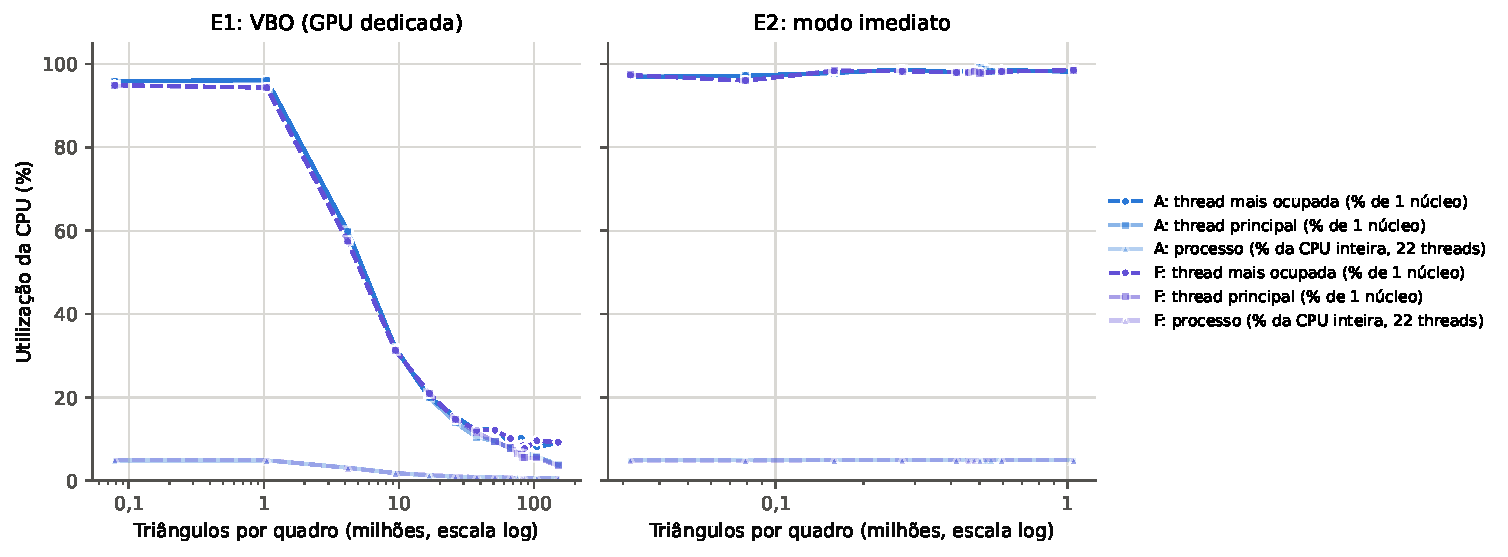
\includegraphics[width=\textwidth]{g5_cpu.pdf}
\caption{Utilização da CPU $\times$ triângulos (configurações A e F). ``Thread mais ocupada'' e
``thread principal'' em \% de um núcleo; ``processo'' em \% da CPU inteira (22 threads lógicas),
como no Gerenciador de Tarefas. À direita, o mesmo para o modo imediato (E2).}
\label{fig:g5}
\end{figure}

\begin{figure}[H]
\centering
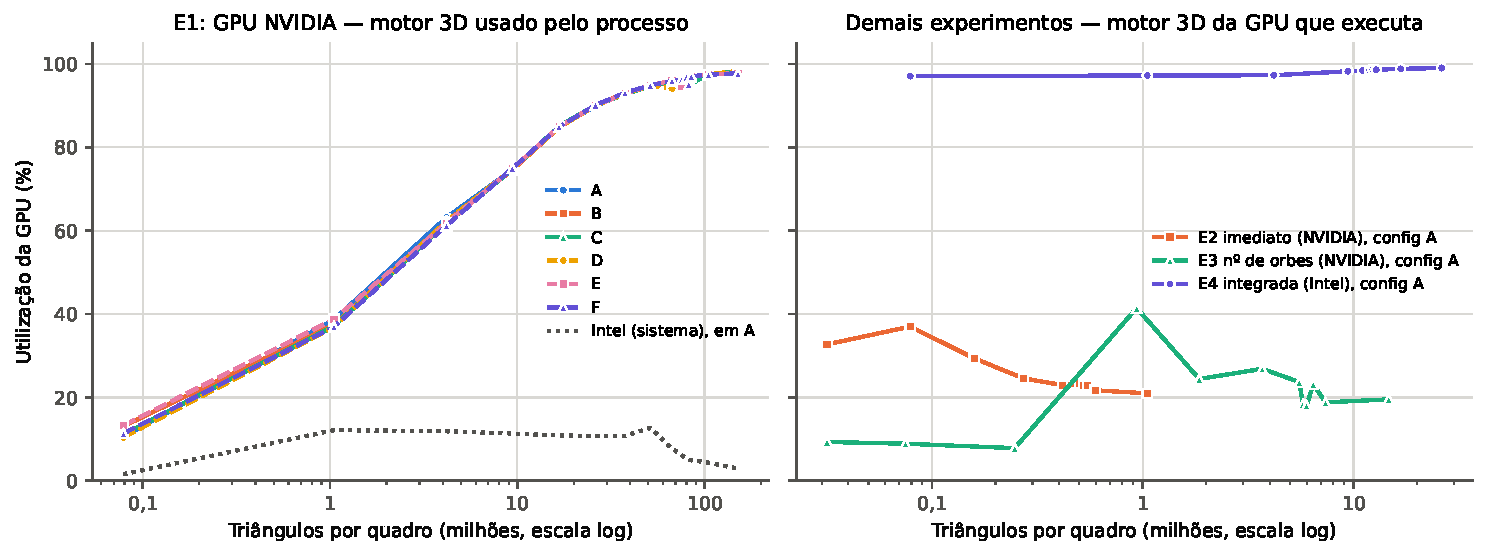
\includegraphics[width=\textwidth]{g6_gpu.pdf}
\caption{Utilização do motor 3D da GPU pelo processo (contadores PDH) $\times$ triângulos. À
esquerda, a NVIDIA no E1 (e a Intel, que só compõe a tela); à direita, a GPU que desenha em cada
um dos demais experimentos.}
\label{fig:g6}
\end{figure}

\begin{figure}[H]
\centering
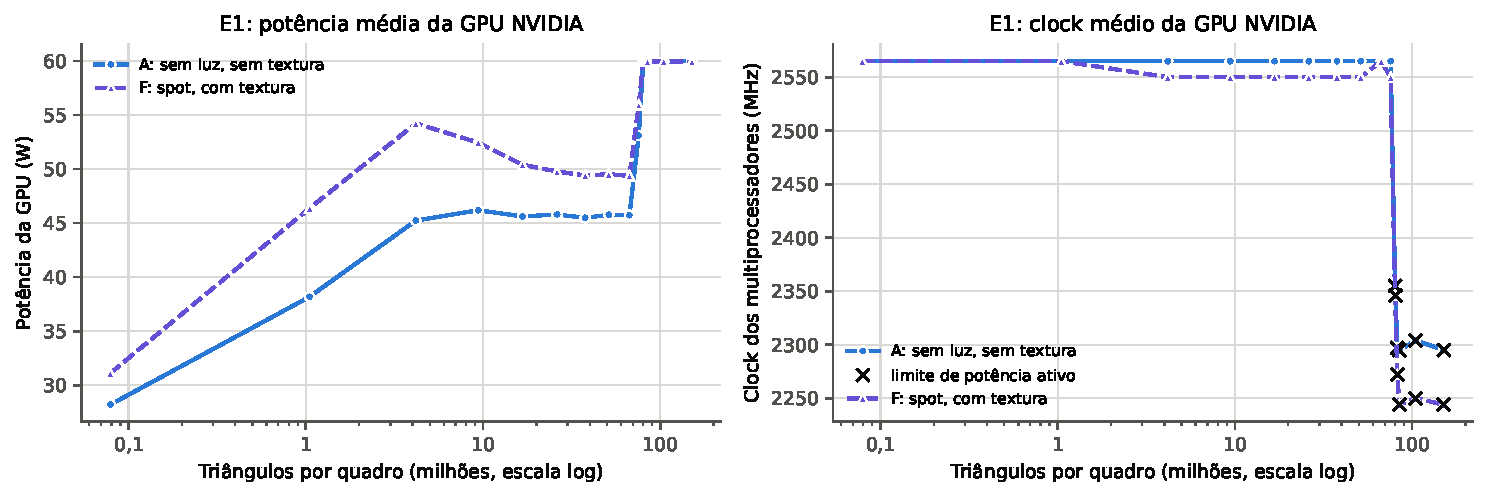
\includegraphics[width=\textwidth]{g7_potencia_clock.pdf}
\caption{Potência e clock dos multiprocessadores da GPU NVIDIA no E1 (NVML). Os ``$\times$''
marcam os pontos em que o NVML informou redução de clock por limite de potência.}
\label{fig:g7}
\end{figure}

No E1 a utilização da CPU pelo processo nunca passou de 5\% da CPU inteira, e no limite de 60~FPS
ficou abaixo de 1\% (Figura~\ref{fig:g5}). Em \% de um núcleo, a thread principal vai de
$\approx$96\% nas cargas leves a menos de 10\% nas cargas altas. Ou seja, quanto mais pesada a
cena, \emph{menos} a CPU trabalha, porque ela passa a maior parte do quadro esperando a GPU. Já a
utilização do motor 3D da NVIDIA sobe de 11\% para 95--98\% (Figura~\ref{fig:g6}). A potência
estabiliza em $\approx$46~W entre 9 e 67 milhões de triângulos e sobe para o limite de
\textbf{60~W} a partir de 80 milhões, quando o \emph{driver} passa a reduzir o clock de 2\,565 para
$\approx$2\,300~MHz (Figura~\ref{fig:g7}). A temperatura ficou entre 64 e 74~$^\circ$C, sem redução
térmica.

% ===========================================================================
\section{Investigação dos gargalos}
\label{sec:gargalos}
% ===========================================================================

\subsection{Decomposição do tempo do quadro}

A Figura~\ref{fig:g8} decompõe o tempo médio de cada quadro (configuração A) em tempo de GPU
(\code{GL_TIME_ELAPSED}), tempo de CPU efetivamente gasto pela thread principal e tempo de
emissão dos comandos. É a evidência mais direta de qual recurso determina o FPS: o quadro não pode
ser mais rápido que o recurso mais lento, então a curva que \emph{coincide} com o tempo total
indica o limitante.

\begin{figure}[H]
\centering
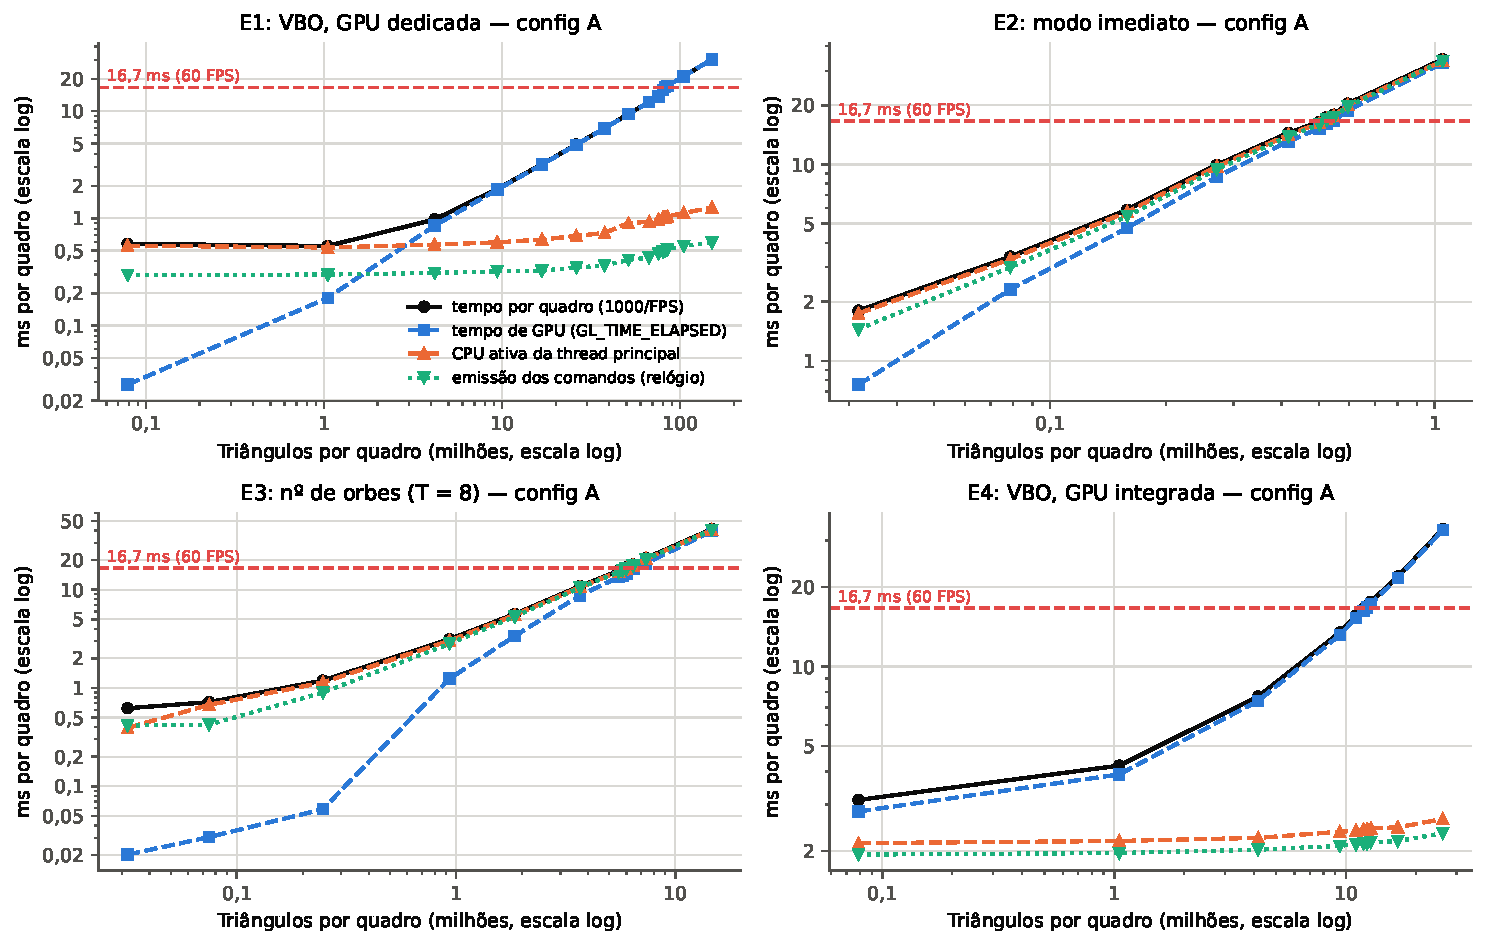
\includegraphics[width=\textwidth]{g8_tempos_quadro.pdf}
\caption{Decomposição do tempo por quadro nos quatro experimentos (configuração A). A linha
tracejada vermelha é o orçamento de 16,7~ms de um quadro a 60~FPS.}
\label{fig:g8}
\end{figure}

\paragraph{E1, cargas leves (até $\approx$1 milhão de triângulos): limite da CPU.}
Com $T=16$ o quadro dura 0,58~ms, dos quais 0,56~ms são CPU ativa da thread principal, enquanto a
GPU trabalha só 0,03~ms. A GPU fica ociosa 95\% do tempo (utilização de 11\%) e a thread principal
está a 96\% de um núcleo. Nessa região o custo é fixo por quadro (67 chamadas de desenho, troca de
\emph{shaders} e \emph{uniforms}, troca de \emph{buffers} e a cópia do quadro para a GPU integrada
via Optimus), por isso o FPS não depende dos triângulos. A sensibilidade desse regime ao clock e ao
escalonamento da CPU explica as diferenças de até 10\% entre execuções observadas no
re-teste da configuração F.

\paragraph{E1, cargas médias e altas: limite da GPU (processamento de geometria).}
A partir de $T=192$ (9,4 milhões) o tempo de GPU coincide com o tempo do quadro (1,85 de 1,88~ms;
16,68 de 16,71~ms no limite), enquanto a CPU ativa cresce só de 0,6 para 1,0~ms. A GPU passa
99,8\% do quadro trabalhando; a CPU, menos de 7\%. Como o FPS cai na proporção inversa dos
triângulos e não depende da iluminação nem da textura (Seção~\ref{sec:luz_textura}), o trabalho
limitante está no \textbf{processamento de vértices e na montagem/rasterização de triângulos}, não
nos fragmentos. Isso é coerente com a geometria: no limite são 82 milhões de triângulos numa
janela de 0,92 milhão de pixels, ou seja, a imensa maioria dos triângulos é menor que um pixel e
não gera fragmento nenhum, mas todos os seus vértices precisam ser transformados. A vazão medida
é de $\approx$5,5 bilhões de triângulos por segundo a 2\,565~MHz (67,0 milhões em 12,18~ms).

\paragraph{O ``joelho'' perto de 60~FPS: memória e limite de potência.}
Até $T=512$ o controlador de memória da GPU fica praticamente parado (0--1\% no NVML), mesmo com
a GPU 100\% ocupada. Isso acontece porque os 64 orbes compartilham \emph{uma única} malha, que é
lida 64 vezes por quadro. Com $T=512$ essa malha (vértices de 32 bytes mais índices de 32 bits)
ocupa $\approx$28~MB, e a cada orbe ela é relida de dentro da cache L2 da GPU. Com $T=544$
(31,6~MB) a utilização da memória sobe para 13\%; com $T=560$ (33,5~MB), para 57\%; e a partir
daí fica em 67--68\%. A malha deixou de caber na cache L2, cuja capacidade no chip AD107 é da
ordem de 32~MB, e passou a ser buscada na memória GDDR6 a cada orbe. O tráfego de memória eleva o
consumo, a GPU atinge o limite de 60~W, e o \emph{driver} reduz o clock em 10\% (2\,565
$\to$ 2\,297~MHz) para respeitar esse limite. A vazão cai na mesma proporção: 4,94 bilhões de
triângulos por segundo no ponto do limite, 0,898 da anterior, contra a razão de clocks de 0,896.

Ou seja, o FPS de 60 é atingido exatamente quando o sistema troca de regime: antes, limite de
\emph{processamento} da GPU com dados na cache; depois, limite de \emph{potência} da GPU
provocado pelo acesso à memória. Isso também explica por que as seis configurações cruzam os
60~FPS no mesmo ponto: a transição depende do tamanho da malha, que é o mesmo em todas.

\subsection{Teste das hipóteses: levando o gargalo para a CPU (E2 e E3)}

Se o E1 é limitado pela GPU, transferir trabalho para a CPU deve mudar completamente o limite e
os indicadores. Os experimentos E2 e E3 fazem isso de duas formas.

\begin{figure}[H]
\centering
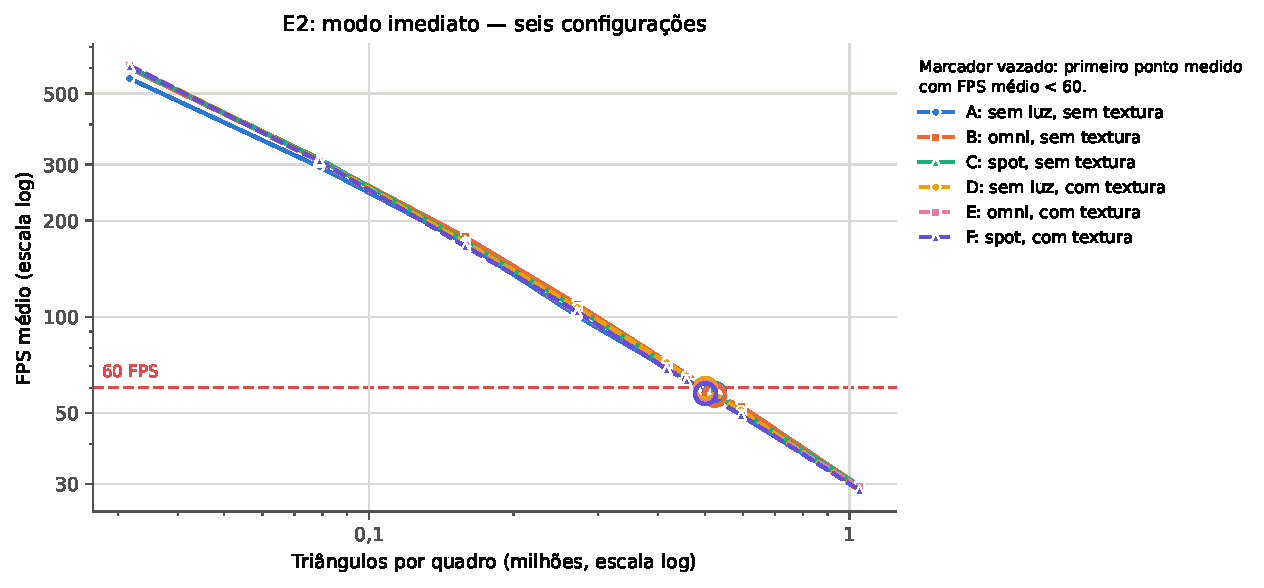
\includegraphics[width=0.92\textwidth]{g10_fps_imediato.pdf}
\caption{E2: modo imediato (\code{glBegin}/\code{glEnd}), seis configurações.}
\label{fig:g10}
\end{figure}

\begin{table}[H]
\centering
\caption{Tabela-síntese do experimento E2 (modo imediato, GPU dedicada).}
\label{tab:sintese_e2}
\scriptsize
\setlength{\tabcolsep}{3pt}
\begin{tabularx}{\textwidth}{c r r r c c L P{1.6cm}}
\toprule
Cfg. & Último $\geq$ 60 & \textbf{Menor testado} & FPS médio & CPU proc. / & GPU 3D & Gargalo & Situação \\
 & (FPS) & \textbf{$<$ 60} & $\pm$ dp & thread máx. (\%) & (\%) & (indício mais forte) & \\
\midrule
A & 501.776 (60,8) & \textbf{524.304} & \textbf{57,6} $\pm$ 0,42 & 5,0 / 99 & 23 & CPU: 1 thread saturada (envio de comandos) & limite encontrado \\
B & 501.776 (60,5) & \textbf{524.304} & \textbf{56,8} $\pm$ 1,13 & 5,0 / 98 & 23 & CPU: 1 thread saturada (envio de comandos) & limite encontrado \\
C & 479.760 (62,8) & \textbf{501.776} & \textbf{59,7} $\pm$ 0,00 & 5,0 / 99 & 23 & CPU: 1 thread saturada (envio de comandos) & limite encontrado \\
D & 479.760 (60,8) & \textbf{501.776} & \textbf{59,8} $\pm$ 0,31 & 4,9 / 98 & 23 & CPU: 1 thread saturada (envio de comandos) & limite encontrado \\
E & 479.760 (61,5) & \textbf{501.776} & \textbf{58,3} $\pm$ 0,49 & 4,9 / 97 & 20 & CPU: 1 thread saturada (envio de comandos) & limite encontrado \\
F & 479.760 (60,9) & \textbf{501.776} & \textbf{57,5} $\pm$ 0,06 & 4,9 / 98 & 20 & CPU: 1 thread saturada (envio de comandos) & limite encontrado \\
\bottomrule
\end{tabularx}
\end{table}


\paragraph{E2, modo imediato.}
Cada vértice de cada triângulo passa a ser enviado pela CPU a cada quadro, com três chamadas de
função (\code{glTexCoord2f}, \code{glNormal3f}, \code{glVertex3f}). O limite de 60~FPS cai para
$\approx$\textbf{0,5 milhão} de triângulos (\limImedA{} na configuração A), \textbf{160 vezes
menos} que com VBO. Os indicadores se invertem em relação ao E1 (Figuras~\ref{fig:g5},
\ref{fig:g6} e \ref{fig:g8}): uma thread do processo fica a 97--99\% de um núcleo, a CPU ativa
(16,4--17,3~ms) ocupa todo o quadro, e a GPU NVIDIA fica só 20--23\% ocupada, com o clock
reduzido pelo próprio \emph{driver} por falta de trabalho em parte das execuções. O custo é de
$\approx$3,6~ns por chamada (524\,304 triângulos $\times$ 3 vértices $\times$ 3 chamadas em
17~ms). A utilização do \emph{processo}, $\approx$5\% da CPU, é praticamente uma thread em 22
($100/22 = 4{,}5\%$): o gargalo de CPU é invisível olhando só para o total.

Neste regime, o tempo medido por \code{GL_TIME_ELAPSED} quase coincide com o do quadro (gráfico
E2 da Figura~\ref{fig:g8}), mas a utilização da GPU é de 23\%. Isso acontece porque a consulta mede o
intervalo entre o início e o fim dos comandos \emph{na linha do tempo da GPU}, incluindo os
períodos em que ela esperava os comandos chegarem. Por isso o critério de gargalo usa os dois
indicadores juntos.

\begin{figure}[H]
\centering
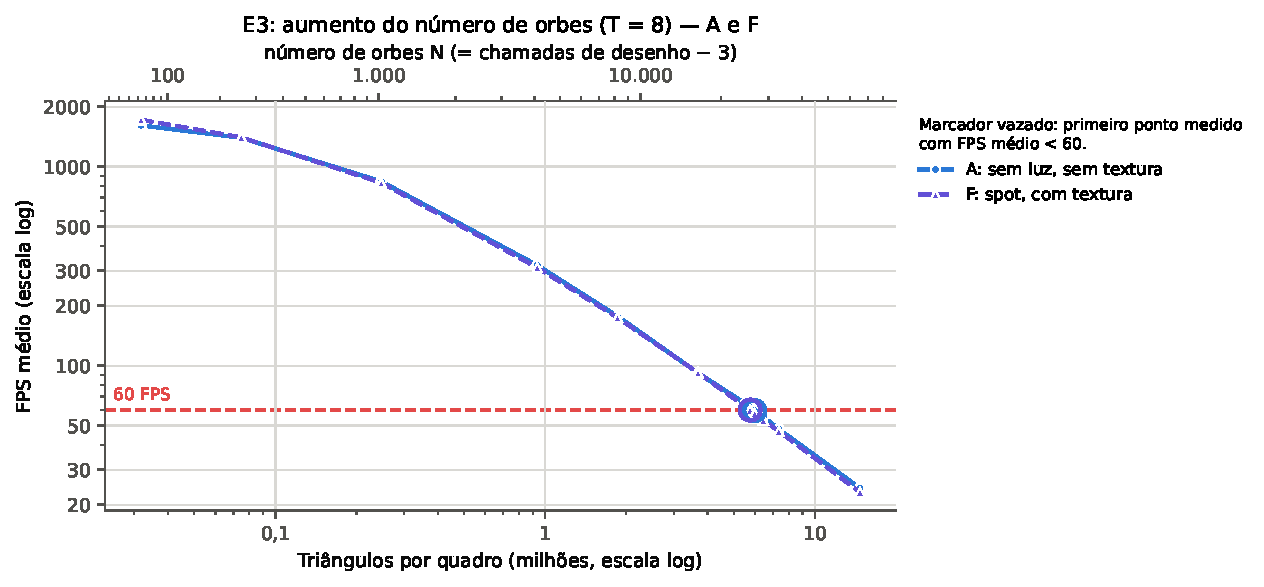
\includegraphics[width=0.92\textwidth]{g11_fps_objetos.pdf}
\caption{E3: aumento do número de orbes $N$ (cada um uma chamada de desenho), $T=8$. O eixo
superior mostra $N$.}
\label{fig:g11}
\end{figure}

\begin{table}[H]
\centering
\caption{Tabela-síntese do experimento E3 (aumento do número de orbes, T = 8).}
\label{tab:sintese_e3}
\scriptsize
\setlength{\tabcolsep}{3pt}
\begin{tabularx}{\textwidth}{c r r r c c L P{1.6cm}}
\toprule
Cfg. & Último $\geq$ 60 & \textbf{Menor testado} & FPS médio & CPU proc. / & GPU 3D & Gargalo & Situação \\
 & (FPS) & \textbf{$<$ 60} & $\pm$ dp & thread máx. (\%) & (\%) & (indício mais forte) & \\
\midrule
A & 5.751.824 (61,9) & \textbf{5.981.200} & \textbf{59,4} $\pm$ 0,33 & 4,9 / 97 & 18 & CPU: 1 thread saturada (envio de comandos) & limite encontrado \\
F & 5.522.448 (62,1) & \textbf{5.751.824} & \textbf{59,8} $\pm$ 0,06 & 4,9 / 99 & 19 & CPU: 1 thread saturada (envio de comandos) & limite encontrado \\
\bottomrule
\end{tabularx}
\end{table}


\paragraph{E3, muitos objetos.}
Com orbes de apenas 224 triângulos, o limite de 60~FPS é atingido com $N\approx$ 26 mil orbes,
ou \textbf{6 milhões} de triângulos (\limObjA{} em A). No E1, os mesmos 6 milhões de triângulos
divididos em 64 objetos rodam a $\approx$750~FPS. A diferença está no número de chamadas de
desenho: cada orbe exige o envio da matriz de modelagem, da cor e um \code{glDrawElements}, e
custa $\approx$0,6~µs de CPU (16,4~ms / 26\,627 chamadas). Novamente uma thread fica a 97--99\%,
a GPU a 18--19\%, e iluminação e textura são irrelevantes. Ao aumentar $N$ o gargalo é o número
de objetos (custo de CPU por chamada), não o de polígonos.

\subsection{Mesma aplicação, GPU integrada (E4)}

\begin{figure}[H]
\centering
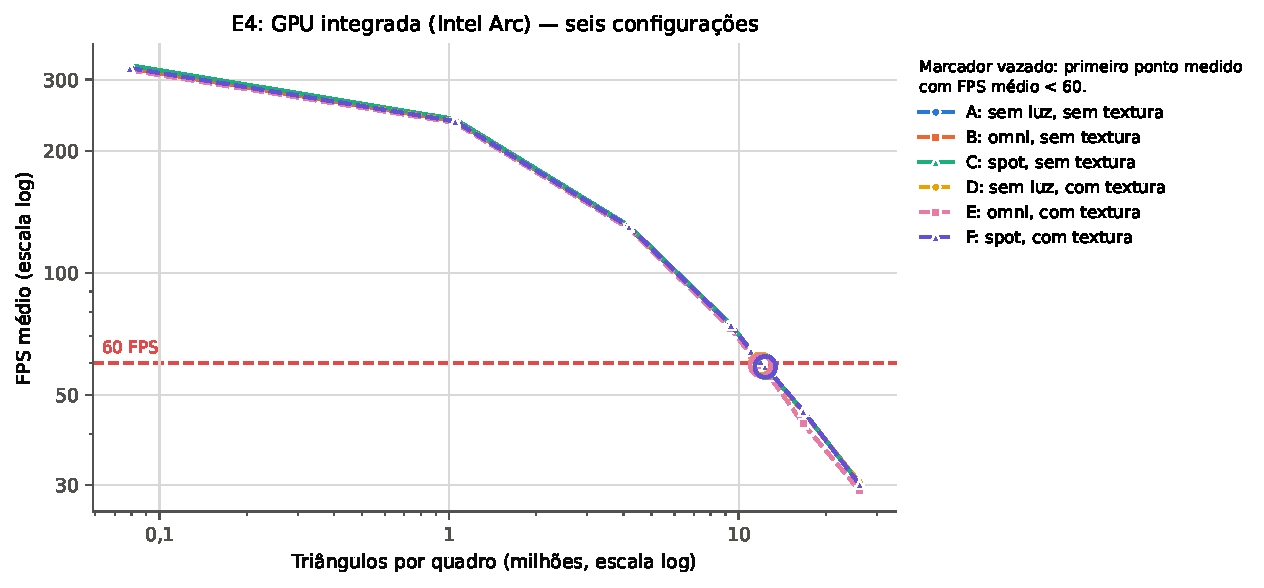
\includegraphics[width=0.92\textwidth]{g12_fps_integrada.pdf}
\caption{E4: a mesma varredura do E1 executada na GPU integrada Intel Arc.}
\label{fig:g12}
\end{figure}

\begin{table}[H]
\centering
\caption{Tabela-síntese do experimento E4 (GPU integrada Intel Arc, VBO, aumento de T).}
\label{tab:sintese_e4}
\scriptsize
\setlength{\tabcolsep}{3pt}
\begin{tabularx}{\textwidth}{c r r r c c L P{1.6cm}}
\toprule
Cfg. & Último $\geq$ 60 & \textbf{Menor testado} & FPS médio & CPU proc. / & GPU 3D & Gargalo & Situação \\
 & (FPS) & \textbf{$<$ 60} & $\pm$ dp & thread máx. (\%) & (\%) & (indício mais forte) & \\
\midrule
A & 11.906.064 (60,5) & \textbf{12.351.504} & \textbf{58,8} $\pm$ 0,04 & 0,9 / 15 & 99 & GPU (processamento de vértices) & limite encontrado \\
B & 11.906.064 (60,5) & \textbf{12.351.504} & \textbf{58,5} $\pm$ 0,08 & 0,8 / 14 & 98 & GPU (processamento de vértices) & limite encontrado \\
C & 11.906.064 (60,6) & \textbf{12.351.504} & \textbf{58,6} $\pm$ 0,12 & 0,9 / 14 & 98 & GPU (processamento de vértices) & limite encontrado \\
D & 11.468.816 (62,3) & \textbf{11.906.064} & \textbf{59,6} $\pm$ 0,07 & 0,9 / 15 & 98 & GPU (processamento de vértices) & limite encontrado \\
E & 11.468.816 (61,0) & \textbf{11.906.064} & \textbf{59,1} $\pm$ 0,08 & 0,9 / 15 & 96 & GPU (processamento de vértices) & limite encontrado \\
F & 11.906.064 (60,6) & \textbf{12.351.504} & \textbf{58,7} $\pm$ 0,11 & 0,8 / 14 & 99 & GPU (processamento de vértices) & limite encontrado \\
\bottomrule
\end{tabularx}
\end{table}


Na GPU integrada, o limite fica entre \textbf{11,9 e 12,4 milhões} de triângulos, $\approx$6,7
vezes menos que na RTX 4060. O motor 3D da Intel fica a 96--99\% desde as cargas mais leves e o
tempo de GPU coincide com o do quadro em toda a faixa (Figura~\ref{fig:g8}): é um gargalo de GPU
puro, e a CPU ativa fica em $\approx$2,1--2,4~ms por quadro (14--15\% de um núcleo). Diferente da
NVIDIA, a Intel tem um custo fixo de $\approx$2,8~ms por quadro mesmo com 79 mil triângulos, o
mesmo em A e em F, que limita o FPS máximo a $\approx$320. Descontado esse custo fixo, a vazão de
geometria é de $\approx$0,9 bilhão de triângulos por segundo, cerca de 6 vezes menor que a da RTX.
O \emph{driver} da Intel também gasta $\approx$4 vezes mais CPU por quadro que o da NVIDIA
(2,1 contra 0,55~ms), sem que isso chegue a limitar o FPS.

\subsection{Síntese dos regimes}

\begin{figure}[H]
\centering
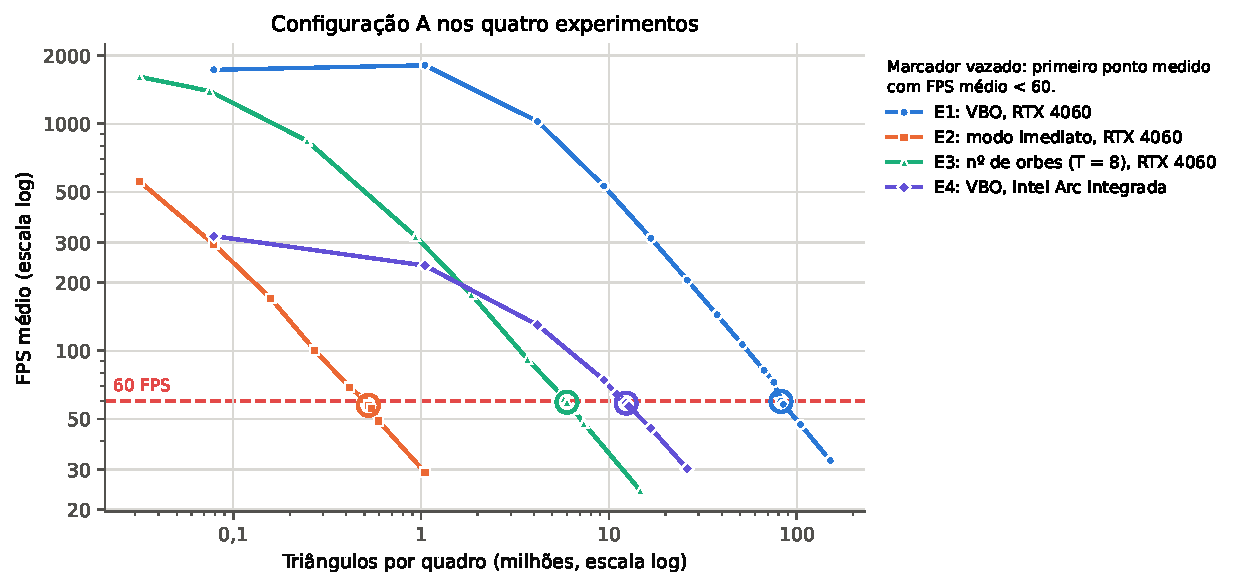
\includegraphics[width=\textwidth]{g9_regimes.pdf}
\caption{Configuração A nos quatro experimentos: a mesma cena atinge 60~FPS com 0,5 a 82 milhões
de triângulos, conforme onde está o gargalo.}
\label{fig:g9}
\end{figure}

\begin{table}[H]
\centering
\caption{Gargalo identificado em cada experimento, no ponto do limite de 60~FPS (configuração A).}
\label{tab:regimes}
\footnotesize
\setlength{\tabcolsep}{4pt}
\begin{tabular}{l r c c c P{3.6cm}}
\toprule
Exp. & Limite (triâng.) & Thread máx. & GPU 3D & GPU/quadro & Gargalo \\
\midrule
E1 VBO, RTX & \limVboA & \thrVboA\% & \gpuVboA\% & 99,8\% & GPU: geometria; malha fora da cache L2 e limite de potência (60~W) \\
E2 imediato, RTX & \limImedA & \thrImedA\% & \gpuImedA\% & -- & CPU: uma thread emitindo vértice a vértice \\
E3 $N$ orbes, RTX & \limObjA & \thrObjA\% & \gpuObjA\% & -- & CPU: uma thread emitindo uma chamada de desenho por objeto \\
E4 VBO, Intel & \limIntA & \thrIntA\% & \gpuIntA\% & 98,3\% & GPU integrada: geometria \\
\bottomrule
\end{tabular}
\end{table}

Em resumo, com a geometria em VBO e poucos objetos, que é a forma recomendada de usar o OpenGL
moderno, a CPU praticamente não participa e o limite de 60~FPS é imposto pela GPU. O mesmo número de
polígonos pode, no entanto, ficar limitado pela CPU se for enviado de forma ineficiente (modo
imediato) ou fragmentado em muitos objetos. Em nenhum caso a utilização total da CPU passou de
5\%: o gargalo de CPU, quando existe, é de \emph{uma} thread.

% ===========================================================================
\section{Influência da iluminação e das texturas}
\label{sec:luz_textura}
% ===========================================================================

A Tabela~\ref{tab:luz_textura} mostra a variação do FPS de cada configuração em relação à A, no
E1, em três cargas típicas.

\begin{table}[H]
\centering
\caption{Variação do FPS em relação à configuração A no E1 (positivo = mais rápido que A).}
\label{tab:luz_textura}
\footnotesize
\begin{tabular}{l r r r r r r}
\toprule
Carga & FPS de A & B & C & D & E & F \\
\midrule
$T=64$ (1,0 milhão, limite da CPU) & 1\,811 & $-9{,}3\%$ & $-7{,}0\%$ & $-6{,}3\%$ & $-7{,}7\%$ & $-9{,}6\%$ \\
$T=256$ (16,7 milhões, GPU) & 313,5 & $-0{,}2\%$ & $-0{,}7\%$ & $-0{,}1\%$ & $-0{,}9\%$ & $-0{,}7\%$ \\
$T=568$ (82,5 milhões, limite) & 59,8 & $-2{,}3\%$ & $-2{,}3\%$ & $-1{,}0\%$ & $-3{,}2\%$ & $-1{,}7\%$ \\
\bottomrule
\end{tabular}
\end{table}

\begin{itemize}
  \item \textbf{Na região limitada pela GPU, a iluminação e as texturas custam menos de 1\%.} A
        iluminação é calculada por fragmento e a textura é lida por fragmento, e o número de
        fragmentos é limitado pelo tamanho da janela (0,92 milhão de pixels), não pelos
        triângulos. O custo total medido pela GPU de iluminar e texturizar a tela inteira é de
        apenas 0,01--0,02~ms por quadro: com $T=16$, o tempo de GPU é 0,028~ms em A e
        0,040--0,047~ms em B, E e F. Diante de 16,7~ms de geometria, é desprezível.
  \item \textbf{O spot não é mais caro que a luz omnidirecional} de forma mensurável: o teste do
        cone (\code{smoothstep} sobre o cosseno do ângulo) acrescenta poucas operações por
        fragmento, e fora do cone o termo especular é zerado.
  \item \textbf{No limite de 60~FPS as diferenças chegam a 1--3\%}, com A sempre a mais rápida.
        Essa diferença, um pouco maior que nas cargas médias, aparece justamente quando a malha sai
        da cache e o limite de potência entra em ação. Uma explicação plausível é que, nas variantes
        que usam iluminação ou textura, a GPU precisa transportar para a rasterização mais dados
        por vértice (posição no espaço do observador, normal, coordenada de textura), enquanto na A
        o compilador pode eliminar essas saídas. Não alteram o ponto de cruzamento.
  \item \textbf{Na região limitada pela CPU} as diferenças de 6--10\% não têm relação com o
        custo das configurações, já que a GPU trabalha menos de 0,2~ms em todas. Elas estão dentro da
        variação entre execuções desse regime (10\% entre as duas execuções da F com $T=16$). No
        E2, também limitado pela CPU, as configurações com iluminação e textura chegaram a ser
        até 10\% \emph{mais} rápidas que a A, o que confirma que as diferenças ali são ruído.
  \item \textbf{Na GPU integrada} (E4), as diferenças ficam em geral abaixo de 2,5\% (a maior foi de 6,9\%, na E com $T=256$) e o limite de A, B, C e F
        é o mesmo; D e E cruzaram um passo antes (11,9 em vez de 12,4 milhões), com FPS de 59,6 e
        59,1, a menos de 1~FPS da linha.
\end{itemize}
A iluminação e as texturas, portanto, \textbf{não mudam o limite de polígonos} nesta cena. Seu
custo seria relevante numa cena limitada por fragmentos: resolução maior, objetos que ocupem muitos
pixels, muitas luzes ou sobreposição de superfícies transparentes. Com o aumento de polígonos
proposto pela atividade, a carga cresce por vértice, e a geometria domina.

% ===========================================================================
\section{Conclusão}
% ===========================================================================

A aplicação desenvolvida permitiu controlar e contar exatamente os triângulos por quadro,
alternar entre as seis configurações de iluminação e textura e registrar, para cada ponto, o FPS
e a utilização de CPU e GPU, seguindo um protocolo automatizado (2~s de estabilização, 3
repetições de 10~s, V-Sync desligado, janela fixa de $1280\times720$).

\begin{itemize}
  \item No experimento principal (GPU dedicada, VBO), \textbf{as seis configurações ficam abaixo
        de 60~FPS a partir de \limVboA{} triângulos por quadro} ($T=568$), com 80\,155\,664
        triângulos ainda acima de 60~FPS.
  \item O gargalo é a \textbf{GPU}: tempo de GPU igual ao tempo do quadro, motor 3D a 95--97\%,
        CPU do processo abaixo de 1\%. O ponto exato do limite coincide com a saída da malha da
        cache L2, que provoca o aumento do tráfego de memória, o limite de potência de 60~W e uma
        redução de 10\% no clock.
  \item \textbf{Iluminação e texturas influenciam muito pouco} (menos de 1\% na maior parte da
        faixa e até 3\% no limite), porque o custo delas é proporcional aos pixels, enquanto o
        custo que cresce é proporcional aos vértices.
  \item O mesmo limite pode ser 160 vezes menor quando a CPU vira gargalo (modo imediato:
        0,5 milhão) ou 14 vezes menor quando o trabalho é dividido em muitos objetos (6 milhões em
        26 mil chamadas de desenho). Nesses casos, uma única thread fica saturada enquanto a
        utilização total da CPU não passa de 5\%.
  \item Na GPU integrada, o limite é de $\approx$12 milhões de triângulos, 6,7 vezes menor, e
        também limitado pela GPU.
\end{itemize}
As medições mostram que ``utilização alta'' sozinha não identifica o gargalo: foi preciso cruzar
a utilização por thread e por GPU, o tempo do quadro decomposto em tempo de GPU e de CPU e o
comportamento do FPS sob mudanças dirigidas da carga.

% ===========================================================================
\section*{Apêndice --- Todos os pontos medidos}
\addcontentsline{toc}{section}{Apêndice --- Todos os pontos medidos}
% ===========================================================================

Valores médios das 3 repetições de cada ponto. Os dados por repetição estão em
\code{resultados/dados/*_repeticoes.csv}.

{\scriptsize
\setlength{\tabcolsep}{2.6pt}
\begin{longtable}{l r r r r r r r r r r r r}
\caption{Todos os pontos medidos no experimento E1 (médias de 3 repetições de 10 s). ``r'' = ponto de refino; $\blacktriangleright$ = primeiro ponto com FPS médio $<$ 60.}\label{tab:pontos_e1}\\
\toprule
Cfg. & T & Triângulos & FPS & dp & Quadro & GPU & CPU ativa & CPU proc. & Thread máx. & GPU 3D & Pot. & Clock \\
 & & & & & (ms) & (ms) & (ms) & (\%) & (\%) & (\%) & (W) & (MHz) \\
\midrule
\endfirsthead
\toprule
Cfg. & T & Triângulos & FPS & dp & Quadro & GPU & CPU ativa & CPU proc. & Thread máx. & GPU 3D & Pot. & Clock \\
 & & & & & (ms) & (ms) & (ms) & (\%) & (\%) & (\%) & (W) & (MHz) \\
\midrule
\endhead
A & 16 & 78.864 & 1.728,7 & 20,75 & 0,58 & 0,03 & 0,56 & 4,9 & 96 & 11 & 28 & 2.565 \\
A & 64 & 1.049.616 & 1.811,1 & 25,32 & 0,55 & 0,18 & 0,53 & 4,9 & 96 & 39 & 38 & 2.565 \\
A & 128 & 4.178.960 & 1.024,1 & 2,12 & 0,98 & 0,85 & 0,57 & 3,1 & 60 & 63 & 45 & 2.565 \\
A & 192 & 9.405.456 & 532,4 & 0,08 & 1,88 & 1,85 & 0,60 & 1,9 & 32 & 75 & 46 & 2.565 \\
A & 256 & 16.729.104 & 313,5 & 0,04 & 3,19 & 3,17 & 0,63 & 1,3 & 20 & 85 & 46 & 2.565 \\
A & 320 & 26.149.904 & 204,8 & 0,03 & 4,88 & 4,86 & 0,68 & 1,0 & 15 & 90 & 46 & 2.565 \\
A & 384 & 37.667.856 & 144,1 & 0,01 & 6,94 & 6,92 & 0,73 & 0,8 & 12 & 93 & 45 & 2.565 \\
A & 448 & 51.282.960 & 106,5 & 0,01 & 9,39 & 9,36 & 0,90 & 0,8 & 13 & 95 & 46 & 2.565 \\
A & 512 & 66.995.216 & 82,0 & 0,00 & 12,20 & 12,18 & 0,93 & 0,7 & 9 & 96 & 46 & 2.565 \\
A & 544r & 75.637.776 & 72,6 & 0,00 & 13,77 & 13,74 & 0,97 & 0,8 & 10 & 96 & 53 & 2.565 \\
A & 560r & 80.155.664 & 63,2 & 0,05 & 15,83 & 15,80 & 1,02 & 0,6 & 10 & 97 & 60 & 2.355 \\
$\blacktriangleright$A & 568r & 82.463.760 & 59,8 & 0,02 & 16,71 & 16,68 & 1,02 & 0,7 & 8 & 95 & 60 & 2.297 \\
A & 576r & 84.804.624 & 58,1 & 0,06 & 17,21 & 17,19 & 1,04 & 0,7 & 9 & 97 & 60 & 2.295 \\
A & 640 & 104.711.184 & 47,4 & 0,10 & 21,10 & 21,08 & 1,12 & 0,6 & 8 & 97 & 60 & 2.304 \\
A & 768 & 150.815.760 & 32,8 & 0,01 & 30,45 & 30,42 & 1,26 & 0,6 & 9 & 98 & 60 & 2.295 \\
\midrule
B & 16 & 78.864 & 1.718,9 & 45,87 & 0,58 & 0,04 & 0,56 & 5,0 & 95 & 13 & 32 & 2.565 \\
B & 64 & 1.049.616 & 1.642,2 & 25,13 & 0,61 & 0,19 & 0,56 & 4,9 & 93 & 37 & 44 & 2.565 \\
B & 128 & 4.178.960 & 1.006,5 & 2,78 & 0,99 & 0,86 & 0,57 & 3,1 & 59 & 62 & 52 & 2.565 \\
B & 192 & 9.405.456 & 529,9 & 0,12 & 1,89 & 1,86 & 0,58 & 1,8 & 31 & 75 & 52 & 2.565 \\
B & 256 & 16.729.104 & 312,9 & 0,03 & 3,20 & 3,17 & 0,62 & 1,3 & 19 & 85 & 50 & 2.565 \\
B & 320 & 26.149.904 & 204,5 & 0,02 & 4,89 & 4,87 & 0,66 & 1,1 & 14 & 90 & 50 & 2.565 \\
B & 384 & 37.667.856 & 143,9 & 0,01 & 6,95 & 6,93 & 0,74 & 0,9 & 12 & 93 & 49 & 2.565 \\
B & 448 & 51.282.960 & 106,5 & 0,01 & 9,39 & 9,37 & 0,87 & 0,9 & 13 & 95 & 49 & 2.565 \\
B & 512 & 66.995.216 & 81,9 & 0,01 & 12,21 & 12,18 & 0,90 & 0,8 & 10 & 96 & 49 & 2.565 \\
B & 544r & 75.637.776 & 72,2 & 0,04 & 13,86 & 13,83 & 0,96 & 0,7 & 10 & 96 & 56 & 2.551 \\
B & 560r & 80.155.664 & 62,8 & 0,04 & 15,92 & 15,89 & 1,03 & 0,7 & 10 & 97 & 60 & 2.346 \\
$\blacktriangleright$B & 568r & 82.463.760 & 58,5 & 0,04 & 17,11 & 17,08 & 1,05 & 0,7 & 9 & 95 & 60 & 2.245 \\
B & 576r & 84.804.624 & 57,0 & 0,03 & 17,53 & 17,51 & 1,03 & 0,7 & 9 & 97 & 60 & 2.252 \\
B & 640 & 104.711.184 & 46,4 & 0,06 & 21,56 & 21,53 & 1,15 & 0,7 & 9 & 97 & 60 & 2.256 \\
B & 768 & 150.815.760 & 32,3 & 0,01 & 30,97 & 30,94 & 1,22 & 0,6 & 11 & 98 & 60 & 2.254 \\
\midrule
C & 16 & 78.864 & 1.640,4 & 9,19 & 0,61 & 0,04 & 0,57 & 4,9 & 93 & 11 & 32 & 2.565 \\
C & 64 & 1.049.616 & 1.684,8 & 6,70 & 0,59 & 0,19 & 0,56 & 5,0 & 95 & 37 & 45 & 2.565 \\
C & 128 & 4.178.960 & 1.014,1 & 1,67 & 0,99 & 0,85 & 0,55 & 3,0 & 57 & 62 & 53 & 2.563 \\
C & 192 & 9.405.456 & 528,4 & 0,22 & 1,89 & 1,87 & 0,58 & 1,8 & 30 & 75 & 52 & 2.550 \\
C & 256 & 16.729.104 & 311,2 & 0,08 & 3,21 & 3,19 & 0,62 & 1,3 & 18 & 85 & 50 & 2.550 \\
C & 320 & 26.149.904 & 203,3 & 0,02 & 4,92 & 4,89 & 0,66 & 1,1 & 14 & 90 & 49 & 2.550 \\
C & 384 & 37.667.856 & 143,2 & 0,01 & 6,98 & 6,96 & 0,71 & 0,9 & 11 & 93 & 49 & 2.550 \\
C & 448 & 51.282.960 & 105,9 & 0,01 & 9,44 & 9,42 & 0,84 & 0,8 & 11 & 95 & 49 & 2.550 \\
C & 512 & 66.995.216 & 81,9 & 0,01 & 12,21 & 12,19 & 0,88 & 0,8 & 10 & 96 & 49 & 2.565 \\
C & 544r & 75.637.776 & 72,2 & 0,01 & 13,85 & 13,83 & 0,94 & 0,7 & 10 & 96 & 56 & 2.550 \\
C & 560r & 80.155.664 & 62,9 & 0,04 & 15,90 & 15,87 & 1,00 & 0,7 & 10 & 97 & 60 & 2.348 \\
$\blacktriangleright$C & 568r & 82.463.760 & 58,4 & 0,02 & 17,11 & 17,09 & 1,03 & 0,7 & 10 & 97 & 60 & 2.244 \\
C & 576r & 84.804.624 & 57,1 & 0,02 & 17,51 & 17,48 & 1,04 & 0,7 & 9 & 95 & 60 & 2.256 \\
C & 640 & 104.711.184 & 46,4 & 0,03 & 21,53 & 21,51 & 1,14 & 0,7 & 9 & 98 & 60 & 2.258 \\
C & 768 & 150.815.760 & 32,3 & 0,01 & 30,98 & 30,95 & 1,26 & 0,6 & 10 & 98 & 60 & 2.252 \\
\midrule
D & 16 & 78.864 & 1.624,7 & 25,42 & 0,62 & 0,03 & 0,56 & 4,9 & 92 & 10 & 32 & 2.565 \\
D & 64 & 1.049.616 & 1.697,0 & 18,58 & 0,59 & 0,18 & 0,55 & 4,9 & 94 & 37 & 42 & 2.565 \\
D & 128 & 4.178.960 & 1.017,4 & 3,02 & 0,98 & 0,85 & 0,55 & 3,1 & 59 & 62 & 49 & 2.565 \\
D & 192 & 9.405.456 & 530,5 & 0,54 & 1,89 & 1,86 & 0,59 & 1,8 & 31 & 75 & 49 & 2.565 \\
D & 256 & 16.729.104 & 313,1 & 0,02 & 3,19 & 3,17 & 0,63 & 1,3 & 19 & 85 & 47 & 2.565 \\
D & 320 & 26.149.904 & 204,5 & 0,03 & 4,89 & 4,86 & 0,66 & 1,1 & 14 & 90 & 48 & 2.565 \\
D & 384 & 37.667.856 & 143,9 & 0,00 & 6,95 & 6,92 & 0,72 & 0,9 & 12 & 93 & 47 & 2.565 \\
D & 448 & 51.282.960 & 106,3 & 0,00 & 9,40 & 9,38 & 0,84 & 0,9 & 11 & 95 & 47 & 2.565 \\
D & 512 & 66.995.216 & 81,9 & 0,00 & 12,21 & 12,19 & 0,89 & 0,7 & 10 & 94 & 47 & 2.565 \\
D & 544r & 75.637.776 & 72,2 & 0,00 & 13,86 & 13,84 & 0,95 & 0,7 & 10 & 96 & 55 & 2.550 \\
D & 560r & 80.155.664 & 63,8 & 0,04 & 15,69 & 15,66 & 0,99 & 0,8 & 15 & 97 & 60 & 2.378 \\
$\blacktriangleright$D & 568r & 82.463.760 & 59,3 & 0,02 & 16,87 & 16,84 & 1,07 & 0,7 & 10 & 97 & 60 & 2.276 \\
D & 576r & 84.804.624 & 57,6 & 0,03 & 17,38 & 17,35 & 1,04 & 0,7 & 10 & 97 & 60 & 2.271 \\
D & 640 & 104.711.184 & 46,8 & 0,09 & 21,35 & 21,32 & 1,14 & 0,7 & 10 & 97 & 60 & 2.276 \\
D & 768 & 150.815.760 & 32,6 & 0,01 & 30,70 & 30,68 & 1,23 & 0,6 & 9 & 98 & 60 & 2.275 \\
\midrule
E & 16 & 78.864 & 1.658,8 & 28,09 & 0,60 & 0,05 & 0,57 & 5,0 & 95 & 13 & 34 & 2.555 \\
E & 64 & 1.049.616 & 1.672,5 & 12,99 & 0,60 & 0,20 & 0,56 & 5,0 & 94 & 39 & 47 & 2.565 \\
E & 128 & 4.178.960 & 1.000,3 & 1,99 & 1,00 & 0,86 & 0,58 & 3,2 & 60 & 62 & 55 & 2.552 \\
E & 192 & 9.405.456 & 525,6 & 0,20 & 1,90 & 1,88 & 0,60 & 1,9 & 32 & 75 & 54 & 2.550 \\
E & 256 & 16.729.104 & 310,8 & 0,09 & 3,22 & 3,19 & 0,63 & 1,3 & 19 & 85 & 51 & 2.550 \\
E & 320 & 26.149.904 & 203,0 & 0,00 & 4,93 & 4,90 & 0,71 & 1,1 & 15 & 90 & 51 & 2.550 \\
E & 384 & 37.667.856 & 143,0 & 0,00 & 6,99 & 6,97 & 0,74 & 0,9 & 12 & 93 & 51 & 2.550 \\
E & 448 & 51.282.960 & 105,7 & 0,01 & 9,46 & 9,43 & 0,83 & 0,8 & 11 & 95 & 51 & 2.550 \\
E & 512 & 66.995.216 & 81,2 & 0,00 & 12,31 & 12,29 & 0,90 & 0,8 & 10 & 96 & 50 & 2.550 \\
E & 544r & 75.637.776 & 71,8 & 0,01 & 13,93 & 13,90 & 0,94 & 0,7 & 9 & 94 & 58 & 2.550 \\
E & 560r & 80.155.664 & 62,0 & 0,05 & 16,14 & 16,12 & 1,01 & 0,7 & 10 & 97 & 60 & 2.329 \\
$\blacktriangleright$E & 568r & 82.463.760 & 57,9 & 0,05 & 17,27 & 17,24 & 1,05 & 0,7 & 9 & 97 & 60 & 2.239 \\
E & 576r & 84.804.624 & 56,1 & 0,03 & 17,81 & 17,78 & 1,04 & 0,7 & 9 & 97 & 60 & 2.234 \\
E & 640 & 104.711.184 & 45,7 & 0,04 & 21,89 & 21,87 & 1,13 & 0,7 & 10 & 97 & 60 & 2.237 \\
E & 768 & 150.815.760 & 31,8 & 0,05 & 31,42 & 31,40 & 1,22 & 0,6 & 9 & 98 & 60 & 2.238 \\
\midrule
F & 16 & 78.864 & 1.543,2 & 166,61 & 0,65 & 0,04 & 0,61 & 5,0 & 95 & 11 & 31 & 2.565 \\
F & 64 & 1.049.616 & 1.638,1 & 11,55 & 0,61 & 0,19 & 0,57 & 5,0 & 94 & 37 & 46 & 2.565 \\
F & 128 & 4.178.960 & 1.000,7 & 1,48 & 1,00 & 0,85 & 0,57 & 3,1 & 57 & 61 & 54 & 2.550 \\
F & 192 & 9.405.456 & 527,0 & 0,36 & 1,90 & 1,87 & 0,60 & 1,8 & 31 & 75 & 52 & 2.550 \\
F & 256 & 16.729.104 & 311,3 & 0,06 & 3,21 & 3,19 & 0,66 & 1,4 & 21 & 85 & 50 & 2.550 \\
F & 320 & 26.149.904 & 203,5 & 0,01 & 4,91 & 4,89 & 0,71 & 1,1 & 15 & 90 & 50 & 2.550 \\
F & 384 & 37.667.856 & 143,2 & 0,01 & 6,99 & 6,96 & 0,78 & 1,0 & 12 & 93 & 49 & 2.550 \\
F & 448 & 51.282.960 & 105,8 & 0,01 & 9,45 & 9,43 & 0,86 & 0,9 & 12 & 95 & 50 & 2.550 \\
F & 512 & 66.995.216 & 81,8 & 0,00 & 12,23 & 12,21 & 0,95 & 0,8 & 10 & 96 & 49 & 2.565 \\
F & 544r & 75.637.776 & 71,9 & 0,00 & 13,92 & 13,89 & 0,89 & 0,6 & 8 & 96 & 56 & 2.550 \\
F & 560r & 80.155.664 & 62,5 & 0,05 & 16,00 & 15,97 & 0,95 & 0,7 & 9 & 97 & 60 & 2.346 \\
$\blacktriangleright$F & 568r & 82.463.760 & 58,8 & 0,04 & 17,01 & 16,98 & 0,97 & 0,6 & 8 & 95 & 60 & 2.272 \\
F & 576r & 84.804.624 & 56,4 & 0,10 & 17,72 & 17,69 & 1,00 & 0,6 & 8 & 97 & 60 & 2.244 \\
F & 640 & 104.711.184 & 46,0 & 0,10 & 21,74 & 21,71 & 1,09 & 0,7 & 10 & 97 & 60 & 2.250 \\
F & 768 & 150.815.760 & 31,9 & 0,08 & 31,36 & 31,34 & 1,11 & 0,5 & 9 & 98 & 60 & 2.244 \\
\bottomrule
\end{longtable}
}

{\scriptsize
\setlength{\tabcolsep}{2.6pt}
\begin{longtable}{l r r r r r r r r r r r r}
\caption{Pontos medidos no experimento E2 (modo imediato).}\label{tab:pontos_e2}\\
\toprule
Cfg. & T & Triângulos & FPS & dp & Quadro & GPU & CPU ativa & CPU proc. & Thread máx. & GPU 3D & Pot. & Clock \\
 & & & & & (ms) & (ms) & (ms) & (\%) & (\%) & (\%) & (W) & (MHz) \\
\midrule
\endfirsthead
\toprule
Cfg. & T & Triângulos & FPS & dp & Quadro & GPU & CPU ativa & CPU proc. & Thread máx. & GPU 3D & Pot. & Clock \\
 & & & & & (ms) & (ms) & (ms) & (\%) & (\%) & (\%) & (W) & (MHz) \\
\midrule
\endhead
A & 8 & 31.760 & 556,9 & 43,07 & 1,80 & 0,76 & 1,75 & 5,0 & 97 & 33 & 26 & 2.565 \\
A & 16 & 78.864 & 294,9 & 13,76 & 3,40 & 2,31 & 3,30 & 5,0 & 97 & 37 & 25 & 2.565 \\
A & 24 & 158.736 & 170,0 & 2,14 & 5,88 & 4,76 & 5,73 & 5,0 & 98 & 29 & 25 & 2.565 \\
A & 32 & 271.376 & 100,6 & 0,19 & 9,94 & 8,65 & 9,75 & 5,0 & 99 & 25 & 24 & 2.565 \\
A & 40r & 416.784 & 69,1 & 0,24 & 14,47 & 13,10 & 14,16 & 5,0 & 98 & 23 & 24 & 2.565 \\
A & 44r & 501.776 & 60,8 & 0,36 & 16,46 & 15,27 & 16,21 & 5,0 & 99 & 23 & 24 & 2.565 \\
$\blacktriangleright$A & 45r & 524.304 & 57,6 & 0,42 & 17,38 & 16,18 & 17,05 & 5,0 & 99 & 23 & 24 & 2.565 \\
A & 46r & 547.344 & 55,8 & 0,07 & 17,92 & 16,68 & 17,64 & 4,9 & 98 & 23 & 24 & 2.565 \\
A & 48 & 594.960 & 49,0 & 0,97 & 20,39 & 18,85 & 20,09 & 5,0 & 98 & 22 & 24 & 2.561 \\
A & 64 & 1.049.616 & 29,2 & 0,15 & 34,29 & 32,78 & 33,65 & 4,9 & 98 & 21 & 24 & 2.565 \\
\midrule
B & 8 & 31.760 & 598,4 & 4,58 & 1,67 & 0,72 & 1,59 & 4,9 & 96 & 32 & 26 & 2.565 \\
B & 16 & 78.864 & 309,8 & 6,93 & 3,23 & 2,24 & 3,13 & 4,9 & 97 & 38 & 25 & 2.565 \\
B & 24 & 158.736 & 177,7 & 1,28 & 5,63 & 4,63 & 5,47 & 4,9 & 97 & 30 & 25 & 2.565 \\
B & 32 & 271.376 & 109,4 & 0,57 & 9,14 & 8,09 & 8,95 & 4,9 & 98 & 26 & 25 & 2.565 \\
B & 40r & 416.784 & 72,5 & 0,94 & 13,80 & 12,66 & 13,55 & 4,9 & 98 & 24 & 25 & 2.565 \\
B & 44r & 501.776 & 60,5 & 0,91 & 16,53 & 15,31 & 16,14 & 4,9 & 98 & 23 & 25 & 2.565 \\
$\blacktriangleright$B & 45r & 524.304 & 56,8 & 1,13 & 17,60 & 16,30 & 17,26 & 5,0 & 98 & 23 & 25 & 2.565 \\
B & 46r & 547.344 & 55,4 & 0,13 & 18,04 & 16,82 & 17,66 & 4,9 & 98 & 23 & 25 & 2.565 \\
B & 48 & 594.960 & 52,6 & 0,37 & 19,03 & 17,87 & 18,82 & 4,9 & 99 & 23 & 25 & 2.565 \\
B & 64 & 1.049.616 & 29,6 & 0,16 & 33,84 & 32,38 & 33,22 & 5,0 & 99 & 21 & 24 & 2.565 \\
\midrule
C & 8 & 31.760 & 604,7 & 4,24 & 1,65 & 0,73 & 1,60 & 4,9 & 97 & 33 & 26 & 2.565 \\
C & 16 & 78.864 & 312,3 & 1,94 & 3,20 & 2,23 & 3,11 & 4,9 & 98 & 38 & 26 & 2.565 \\
C & 24 & 158.736 & 172,5 & 1,23 & 5,80 & 4,72 & 5,61 & 4,9 & 96 & 30 & 25 & 2.565 \\
C & 32 & 271.376 & 105,9 & 1,27 & 9,44 & 8,28 & 9,22 & 4,9 & 97 & 26 & 25 & 2.565 \\
C & 40r & 416.784 & 71,0 & 0,41 & 14,09 & 12,90 & 13,76 & 4,9 & 97 & 23 & 25 & 2.565 \\
C & 42r & 458.256 & 64,6 & 0,45 & 15,47 & 14,24 & 15,16 & 4,9 & 98 & 23 & 25 & 2.565 \\
C & 43r & 479.760 & 62,8 & 0,12 & 15,93 & 14,72 & 15,59 & 4,9 & 98 & 23 & 25 & 2.565 \\
$\blacktriangleright$C & 44r & 501.776 & 59,7 & 0,00 & 16,75 & 15,54 & 16,43 & 5,0 & 99 & 23 & 25 & 2.565 \\
C & 48 & 594.960 & 50,6 & 0,23 & 19,75 & 18,47 & 19,32 & 4,9 & 97 & 22 & 25 & 2.565 \\
C & 64 & 1.049.616 & 29,5 & 0,30 & 33,85 & 32,41 & 33,24 & 4,9 & 98 & 21 & 24 & 2.565 \\
\midrule
D & 8 & 31.760 & 612,8 & 5,24 & 1,63 & 0,71 & 1,57 & 4,8 & 95 & 32 & 26 & 2.565 \\
D & 16 & 78.864 & 309,0 & 2,03 & 3,24 & 2,26 & 3,15 & 4,9 & 98 & 38 & 25 & 2.565 \\
D & 24 & 158.736 & 171,0 & 1,43 & 5,85 & 4,80 & 5,74 & 5,0 & 98 & 29 & 25 & 2.565 \\
D & 32 & 271.376 & 107,0 & 0,84 & 9,35 & 8,26 & 9,15 & 4,9 & 99 & 26 & 25 & 2.565 \\
D & 40r & 416.784 & 71,9 & 0,13 & 13,91 & 12,76 & 13,64 & 4,9 & 98 & 24 & 25 & 2.565 \\
D & 42r & 458.256 & 65,3 & 0,35 & 15,30 & 14,08 & 14,98 & 4,9 & 98 & 23 & 25 & 2.565 \\
D & 43r & 479.760 & 60,8 & 1,81 & 16,46 & 15,09 & 16,15 & 4,9 & 98 & 22 & 24 & 2.504 \\
$\blacktriangleright$D & 44r & 501.776 & 59,8 & 0,31 & 16,74 & 15,50 & 16,41 & 4,9 & 98 & 23 & 25 & 2.565 \\
D & 48 & 594.960 & 51,0 & 0,38 & 19,63 & 18,35 & 19,32 & 5,0 & 98 & 22 & 25 & 2.565 \\
D & 64 & 1.049.616 & 28,6 & 0,46 & 34,97 & 33,29 & 34,45 & 5,0 & 99 & 20 & 22 & 2.393 \\
\midrule
E & 8 & 31.760 & 612,5 & 1,94 & 1,63 & 0,69 & 1,57 & 4,8 & 95 & 32 & 27 & 2.565 \\
E & 16 & 78.864 & 305,7 & 3,69 & 3,27 & 2,22 & 3,17 & 4,9 & 97 & 36 & 26 & 2.565 \\
E & 24 & 158.736 & 167,6 & 1,37 & 5,97 & 4,80 & 5,82 & 4,9 & 98 & 27 & 21 & 2.269 \\
E & 32 & 271.376 & 102,9 & 0,69 & 9,72 & 8,40 & 9,50 & 5,0 & 98 & 23 & 14 & 1.372 \\
E & 40r & 416.784 & 69,3 & 0,29 & 14,43 & 13,00 & 14,11 & 4,9 & 97 & 20 & 15 & 1.593 \\
E & 42r & 458.256 & 63,7 & 0,45 & 15,69 & 14,28 & 15,40 & 4,9 & 98 & 20 & 15 & 1.607 \\
E & 43r & 479.760 & 61,5 & 0,20 & 16,25 & 14,81 & 15,92 & 4,9 & 98 & 20 & 16 & 1.662 \\
$\blacktriangleright$E & 44r & 501.776 & 58,3 & 0,49 & 17,16 & 15,68 & 16,82 & 4,9 & 97 & 20 & 15 & 1.531 \\
E & 48 & 594.960 & 49,2 & 0,20 & 20,32 & 18,80 & 19,84 & 4,9 & 98 & 20 & 16 & 1.626 \\
E & 64 & 1.049.616 & 29,3 & 0,05 & 34,08 & 32,31 & 33,43 & 4,9 & 99 & 19 & 16 & 1.663 \\
\midrule
F & 8 & 31.760 & 609,4 & 0,78 & 1,64 & 0,66 & 1,57 & 4,9 & 97 & 30 & 27 & 2.565 \\
F & 16 & 78.864 & 307,7 & 2,10 & 3,25 & 2,16 & 3,12 & 4,8 & 96 & 34 & 26 & 2.565 \\
F & 24 & 158.736 & 166,3 & 2,73 & 6,02 & 4,77 & 5,88 & 5,0 & 98 & 26 & 17 & 1.763 \\
F & 32 & 271.376 & 103,6 & 0,41 & 9,65 & 8,37 & 9,46 & 4,9 & 98 & 22 & 14 & 1.409 \\
F & 40r & 416.784 & 68,6 & 0,75 & 14,58 & 13,12 & 14,32 & 4,9 & 98 & 20 & 15 & 1.570 \\
F & 42r & 458.256 & 63,3 & 0,63 & 15,81 & 14,34 & 15,46 & 4,9 & 98 & 20 & 15 & 1.570 \\
F & 43r & 479.760 & 60,9 & 0,23 & 16,43 & 15,02 & 16,07 & 4,9 & 98 & 20 & 15 & 1.542 \\
$\blacktriangleright$F & 44r & 501.776 & 57,5 & 0,06 & 17,39 & 15,91 & 16,98 & 4,9 & 98 & 20 & 16 & 1.671 \\
F & 48 & 594.960 & 49,3 & 0,40 & 20,30 & 18,77 & 19,95 & 4,9 & 98 & 19 & 16 & 1.671 \\
F & 64 & 1.049.616 & 28,7 & 0,10 & 34,86 & 33,03 & 34,25 & 4,9 & 98 & 18 & 15 & 1.598 \\
\bottomrule
\end{longtable}
}

{\scriptsize
\setlength{\tabcolsep}{2.6pt}
\begin{longtable}{l r r r r r r r r r r r r}
\caption{Pontos medidos no experimento E3 (N orbes com T = 8).}\label{tab:pontos_e3}\\
\toprule
Cfg. & N & Triângulos & FPS & dp & Quadro & GPU & CPU ativa & CPU proc. & Thread máx. & GPU 3D & Pot. & Clock \\
 & & & & & (ms) & (ms) & (ms) & (\%) & (\%) & (\%) & (W) & (MHz) \\
\midrule
\endfirsthead
\toprule
Cfg. & N & Triângulos & FPS & dp & Quadro & GPU & CPU ativa & CPU proc. & Thread máx. & GPU 3D & Pot. & Clock \\
 & & & & & (ms) & (ms) & (ms) & (\%) & (\%) & (\%) & (W) & (MHz) \\
\midrule
\endhead
A & 64 & 31.760 & 1.611,1 & 74,81 & 0,62 & 0,02 & 0,39 & 4,8 & 90 & 9 & 26 & 2.565 \\
A & 256 & 74.768 & 1.394,2 & 11,86 & 0,72 & 0,03 & 0,67 & 4,8 & 93 & 9 & 27 & 2.565 \\
A & 1.024 & 246.800 & 841,9 & 9,94 & 1,19 & 0,06 & 1,14 & 4,9 & 96 & 8 & 26 & 2.565 \\
A & 4.096 & 934.928 & 319,1 & 1,55 & 3,13 & 1,25 & 3,02 & 4,8 & 96 & 41 & 14 & 1.170 \\
A & 8.192 & 1.852.432 & 177,3 & 0,90 & 5,64 & 3,38 & 5,52 & 4,9 & 98 & 24 & 13 & 1.060 \\
A & 16.384 & 3.687.440 & 91,9 & 0,10 & 10,89 & 8,77 & 10,61 & 4,9 & 97 & 27 & 10 & 807 \\
A & 24.576r & 5.522.448 & 64,5 & 1,03 & 15,51 & 13,39 & 15,27 & 4,9 & 98 & 24 & 10 & 728 \\
A & 25.600r & 5.751.824 & 61,9 & 0,08 & 16,16 & 14,00 & 15,77 & 4,8 & 96 & 18 & 10 & 719 \\
$\blacktriangleright$A & 26.624r & 5.981.200 & 59,4 & 0,33 & 16,84 & 14,50 & 16,43 & 4,9 & 97 & 18 & 10 & 714 \\
A & 28.672r & 6.439.952 & 55,5 & 0,21 & 18,02 & 16,12 & 17,70 & 5,0 & 99 & 23 & 10 & 669 \\
A & 32.768 & 7.357.456 & 47,9 & 0,64 & 20,88 & 18,52 & 20,56 & 4,9 & 98 & 19 & 10 & 642 \\
A & 65.536 & 14.697.488 & 24,2 & 0,23 & 41,28 & 39,35 & 40,45 & 4,9 & 98 & 20 & 10 & 572 \\
\midrule
F & 64 & 31.760 & 1.718,2 & 21,62 & 0,58 & 0,03 & 0,54 & 4,7 & 92 & 10 & 31 & 2.565 \\
F & 256 & 74.768 & 1.401,7 & 4,31 & 0,71 & 0,04 & 0,67 & 4,8 & 95 & 10 & 31 & 2.565 \\
F & 1.024 & 246.800 & 828,5 & 5,21 & 1,21 & 0,07 & 1,16 & 4,9 & 96 & 9 & 29 & 2.565 \\
F & 4.096 & 934.928 & 310,7 & 0,69 & 3,22 & 1,27 & 3,09 & 4,8 & 97 & 10 & 14 & 1.185 \\
F & 8.192 & 1.852.432 & 174,2 & 3,11 & 5,74 & 3,44 & 5,59 & 4,9 & 97 & 24 & 13 & 1.046 \\
F & 16.384 & 3.687.440 & 92,1 & 0,23 & 10,86 & 8,80 & 10,63 & 4,8 & 96 & 13 & 10 & 796 \\
F & 24.576r & 5.522.448 & 62,1 & 0,18 & 16,09 & 13,95 & 15,77 & 4,9 & 98 & 14 & 10 & 671 \\
$\blacktriangleright$F & 25.600r & 5.751.824 & 59,8 & 0,06 & 16,71 & 14,47 & 16,36 & 4,9 & 99 & 19 & 10 & 667 \\
F & 26.624r & 5.981.200 & 57,4 & 0,73 & 17,41 & 15,05 & 17,15 & 4,9 & 99 & 19 & 10 & 654 \\
F & 28.672r & 6.439.952 & 53,2 & 0,65 & 18,80 & 16,81 & 18,47 & 4,9 & 98 & 20 & 10 & 631 \\
F & 32.768 & 7.357.456 & 46,8 & 0,11 & 21,37 & 18,94 & 20,96 & 4,9 & 98 & 19 & 10 & 628 \\
F & 65.536 & 14.697.488 & 23,1 & 0,21 & 43,24 & 41,05 & 42,45 & 5,0 & 99 & 18 & 10 & 551 \\
\bottomrule
\end{longtable}
}

{\scriptsize
\setlength{\tabcolsep}{2.6pt}
\begin{longtable}{l r r r r r r r r r r r r}
\caption{Pontos medidos no experimento E4 (GPU integrada). Potência e clock da NVML não se aplicam.}\label{tab:pontos_e4}\\
\toprule
Cfg. & T & Triângulos & FPS & dp & Quadro & GPU & CPU ativa & CPU proc. & Thread máx. & GPU 3D & Pot. & Clock \\
 & & & & & (ms) & (ms) & (ms) & (\%) & (\%) & (\%) & (W) & (MHz) \\
\midrule
\endfirsthead
\toprule
Cfg. & T & Triângulos & FPS & dp & Quadro & GPU & CPU ativa & CPU proc. & Thread máx. & GPU 3D & Pot. & Clock \\
 & & & & & (ms) & (ms) & (ms) & (\%) & (\%) & (\%) & (W) & (MHz) \\
\midrule
\endhead
A & 16 & 78.864 & 320,2 & 0,74 & 3,12 & 2,83 & 2,14 & 3,4 & 69 & 97 & -- & -- \\
A & 64 & 1.049.616 & 237,4 & 0,28 & 4,21 & 3,90 & 2,18 & 2,6 & 52 & 97 & -- & -- \\
A & 128 & 4.178.960 & 129,9 & 0,10 & 7,70 & 7,41 & 2,24 & 1,5 & 28 & 97 & -- & -- \\
A & 192 & 9.405.456 & 74,4 & 0,03 & 13,45 & 13,16 & 2,37 & 1,0 & 17 & 98 & -- & -- \\
A & 208r & 11.039.760 & 64,2 & 0,04 & 15,57 & 15,28 & 2,39 & 0,9 & 18 & 98 & -- & -- \\
A & 216r & 11.906.064 & 60,5 & 0,09 & 16,53 & 16,24 & 2,41 & 0,9 & 14 & 98 & -- & -- \\
$\blacktriangleright$A & 220r & 12.351.504 & 58,8 & 0,04 & 17,00 & 16,71 & 2,41 & 0,9 & 15 & 99 & -- & -- \\
A & 224r & 12.805.136 & 56,9 & 0,08 & 17,57 & 17,28 & 2,44 & 0,9 & 14 & 99 & -- & -- \\
A & 256 & 16.729.104 & 45,6 & 0,04 & 21,94 & 21,63 & 2,46 & 0,8 & 12 & 99 & -- & -- \\
A & 320 & 26.149.904 & 30,2 & 0,02 & 33,14 & 32,83 & 2,64 & 0,6 & 8 & 99 & -- & -- \\
\midrule
B & 16 & 78.864 & 319,7 & 1,49 & 3,13 & 2,82 & 2,15 & 3,4 & 67 & 97 & -- & -- \\
B & 64 & 1.049.616 & 237,3 & 0,33 & 4,21 & 3,90 & 2,18 & 2,6 & 52 & 97 & -- & -- \\
B & 128 & 4.178.960 & 130,3 & 0,07 & 7,67 & 7,39 & 2,26 & 1,6 & 30 & 97 & -- & -- \\
B & 192 & 9.405.456 & 74,5 & 0,01 & 13,42 & 13,13 & 2,34 & 1,0 & 18 & 98 & -- & -- \\
B & 208r & 11.039.760 & 64,0 & 0,15 & 15,63 & 15,35 & 2,42 & 1,4 & 28 & 98 & -- & -- \\
B & 216r & 11.906.064 & 60,5 & 0,09 & 16,53 & 16,24 & 2,43 & 0,9 & 15 & 98 & -- & -- \\
$\blacktriangleright$B & 220r & 12.351.504 & 58,5 & 0,08 & 17,09 & 16,80 & 2,43 & 0,8 & 14 & 98 & -- & -- \\
B & 224r & 12.805.136 & 56,9 & 0,15 & 17,57 & 17,27 & 2,46 & 0,8 & 14 & 99 & -- & -- \\
B & 256 & 16.729.104 & 45,6 & 0,06 & 21,94 & 21,64 & 2,51 & 0,8 & 12 & 99 & -- & -- \\
B & 320 & 26.149.904 & 30,3 & 0,04 & 33,05 & 32,74 & 2,67 & 0,5 & 7 & 99 & -- & -- \\
\midrule
C & 16 & 78.864 & 325,6 & 0,73 & 3,07 & 2,77 & 2,10 & 3,3 & 68 & 97 & -- & -- \\
C & 64 & 1.049.616 & 239,7 & 0,34 & 4,17 & 3,87 & 2,17 & 2,6 & 52 & 97 & -- & -- \\
C & 128 & 4.178.960 & 130,8 & 0,08 & 7,65 & 7,35 & 2,22 & 1,6 & 30 & 97 & -- & -- \\
C & 192 & 9.405.456 & 74,6 & 0,12 & 13,41 & 13,10 & 2,34 & 1,0 & 17 & 98 & -- & -- \\
C & 208r & 11.039.760 & 64,3 & 0,08 & 15,54 & 15,25 & 2,37 & 0,9 & 17 & 98 & -- & -- \\
C & 216r & 11.906.064 & 60,6 & 0,03 & 16,49 & 16,18 & 2,35 & 0,9 & 14 & 98 & -- & -- \\
$\blacktriangleright$C & 220r & 12.351.504 & 58,6 & 0,12 & 17,07 & 16,77 & 2,41 & 0,9 & 14 & 98 & -- & -- \\
C & 224r & 12.805.136 & 56,6 & 0,02 & 17,66 & 17,35 & 2,42 & 0,8 & 14 & 99 & -- & -- \\
C & 256 & 16.729.104 & 45,5 & 0,05 & 21,97 & 21,62 & 2,48 & 0,7 & 12 & 99 & -- & -- \\
C & 320 & 26.149.904 & 30,3 & 0,07 & 33,05 & 32,73 & 2,63 & 0,6 & 8 & 99 & -- & -- \\
\midrule
D & 16 & 78.864 & 319,1 & 0,95 & 3,13 & 2,83 & 2,15 & 3,3 & 67 & 97 & -- & -- \\
D & 64 & 1.049.616 & 237,3 & 0,24 & 4,21 & 3,91 & 2,18 & 2,6 & 52 & 97 & -- & -- \\
D & 128 & 4.178.960 & 129,7 & 0,08 & 7,71 & 7,43 & 2,25 & 1,5 & 28 & 97 & -- & -- \\
D & 192 & 9.405.456 & 74,3 & 0,06 & 13,47 & 13,19 & 2,38 & 1,0 & 18 & 98 & -- & -- \\
D & 208r & 11.039.760 & 64,2 & 0,13 & 15,57 & 15,27 & 2,40 & 0,8 & 16 & 98 & -- & -- \\
D & 212r & 11.468.816 & 62,3 & 0,04 & 16,05 & 15,76 & 2,41 & 0,9 & 15 & 98 & -- & -- \\
$\blacktriangleright$D & 216r & 11.906.064 & 59,6 & 0,07 & 16,79 & 16,50 & 2,44 & 0,9 & 15 & 98 & -- & -- \\
D & 224r & 12.805.136 & 56,9 & 0,07 & 17,56 & 17,27 & 2,45 & 0,9 & 15 & 99 & -- & -- \\
D & 256 & 16.729.104 & 45,2 & 0,37 & 22,10 & 21,73 & 2,52 & 0,7 & 11 & 98 & -- & -- \\
D & 320 & 26.149.904 & 30,5 & 0,05 & 32,83 & 32,52 & 2,71 & 0,6 & 8 & 99 & -- & -- \\
\midrule
E & 16 & 78.864 & 316,4 & 1,03 & 3,16 & 2,86 & 2,15 & 3,2 & 65 & 97 & -- & -- \\
E & 64 & 1.049.616 & 234,6 & 0,52 & 4,26 & 3,97 & 2,17 & 2,6 & 52 & 97 & -- & -- \\
E & 128 & 4.178.960 & 128,7 & 0,85 & 7,77 & 7,30 & 2,30 & 1,4 & 27 & 96 & -- & -- \\
E & 192 & 9.405.456 & 72,9 & 0,04 & 13,72 & 13,18 & 2,41 & 1,1 & 18 & 96 & -- & -- \\
E & 208r & 11.039.760 & 62,6 & 0,10 & 15,97 & 15,38 & 2,46 & 0,9 & 16 & 96 & -- & -- \\
E & 212r & 11.468.816 & 61,0 & 0,05 & 16,40 & 15,79 & 2,46 & 0,9 & 16 & 96 & -- & -- \\
$\blacktriangleright$E & 216r & 11.906.064 & 59,1 & 0,08 & 16,91 & 16,24 & 2,47 & 0,9 & 15 & 96 & -- & -- \\
E & 224r & 12.805.136 & 55,5 & 0,09 & 18,02 & 17,30 & 2,50 & 0,9 & 14 & 96 & -- & -- \\
E & 256 & 16.729.104 & 42,4 & 0,07 & 23,58 & 23,02 & 2,56 & 0,7 & 11 & 96 & -- & -- \\
E & 320 & 26.149.904 & 29,0 & 0,30 & 34,43 & 33,71 & 2,68 & 0,6 & 7 & 96 & -- & -- \\
\midrule
F & 16 & 78.864 & 320,4 & 1,51 & 3,12 & 2,81 & 2,13 & 3,4 & 67 & 97 & -- & -- \\
F & 64 & 1.049.616 & 236,7 & 0,32 & 4,22 & 3,92 & 2,15 & 2,6 & 51 & 97 & -- & -- \\
F & 128 & 4.178.960 & 130,1 & 0,05 & 7,69 & 7,40 & 2,23 & 1,5 & 28 & 97 & -- & -- \\
F & 192 & 9.405.456 & 74,4 & 0,02 & 13,44 & 13,15 & 2,35 & 1,1 & 18 & 98 & -- & -- \\
F & 208r & 11.039.760 & 64,2 & 0,11 & 15,57 & 15,29 & 2,39 & 0,8 & 15 & 98 & -- & -- \\
F & 216r & 11.906.064 & 60,6 & 0,03 & 16,50 & 16,21 & 2,39 & 0,9 & 14 & 99 & -- & -- \\
$\blacktriangleright$F & 220r & 12.351.504 & 58,7 & 0,11 & 17,04 & 16,75 & 2,41 & 0,8 & 14 & 99 & -- & -- \\
F & 224r & 12.805.136 & 57,1 & 0,06 & 17,51 & 17,21 & 2,41 & 0,8 & 14 & 99 & -- & -- \\
F & 256 & 16.729.104 & 45,6 & 0,00 & 21,92 & 21,63 & 2,47 & 0,8 & 12 & 99 & -- & -- \\
F & 320 & 26.149.904 & 30,1 & 0,02 & 33,23 & 32,92 & 2,69 & 0,6 & 9 & 99 & -- & -- \\
\bottomrule
\end{longtable}
}



% ===========================================================================
\begin{thebibliography}{99}
\addcontentsline{toc}{section}{Referências bibliográficas}

\bibitem{akenine} AKENINE-MÖLLER, T. et al. \textbf{Real-time rendering}. 4. ed. Boca Raton:
CRC Press, 2018.

\bibitem{redbook} SHREINER, D. et al. \textbf{OpenGL programming guide: the official guide to
learning OpenGL, version 4.3}. 8. ed. Boston: Addison-Wesley, 2013.

\bibitem{glspec} SEGAL, M.; AKELEY, K. \textbf{The OpenGL graphics system: a specification --
version 4.6 (compatibility profile)}. The Khronos Group, 2022. Disponível em:
\url{https://registry.khronos.org/OpenGL/specs/gl/glspec46.compatibility.pdf}. Acesso em: 9 nov. 2026.

\bibitem{glsl} KESSENICH, J. \textbf{The OpenGL Shading Language, version 1.20}. 3Dlabs, 2006.
Disponível em: \url{https://registry.khronos.org/OpenGL/specs/gl/GLSLangSpec.1.20.pdf}. Acesso em:
9 nov. 2026.

\bibitem{hughes} HUGHES, J. F. et al. \textbf{Computer graphics: principles and practice}.
3. ed. Upper Saddle River: Addison-Wesley, 2013.

\bibitem{phong} PHONG, B. T. Illumination for computer generated pictures.
\textbf{Communications of the ACM}, v. 18, n. 6, p. 311--317, 1975.

\bibitem{blinn} BLINN, J. F. Models of light reflection for computer synthesized pictures.
\textbf{ACM SIGGRAPH Computer Graphics}, v. 11, n. 2, p. 192--198, 1977.

\bibitem{williams} WILLIAMS, L. Pyramidal parametrics. \textbf{ACM SIGGRAPH Computer Graphics},
v. 17, n. 3, p. 1--11, 1983.

\bibitem{nvidiaperf} NVIDIA. \textbf{GPU Gems}: chapter 28 -- Graphics pipeline performance.
Disponível em: \url{https://developer.nvidia.com/gpugems/gpugems/part-v-performance-and-practicalities/chapter-28-graphics-pipeline-performance}.
Acesso em: 9 nov. 2026.

\bibitem{timerquery} THE KHRONOS GROUP. \textbf{ARB\_timer\_query}. Disponível em:
\url{https://registry.khronos.org/OpenGL/extensions/ARB/ARB_timer_query.txt}. Acesso em: 9 nov. 2026.

\bibitem{nvml} NVIDIA. \textbf{NVML API reference guide}. Disponível em:
\url{https://docs.nvidia.com/deploy/nvml-api/}. Acesso em: 9 nov. 2026.

\bibitem{pdh} MICROSOFT. \textbf{Performance Counters (PDH)} e \textbf{GPU in Task Manager}.
Disponível em: \url{https://learn.microsoft.com/windows/win32/perfctrs/performance-counters-portal}.
Acesso em: 9 nov. 2026.

\bibitem{optimus} NVIDIA. \textbf{Optimus rendering policies} (NvOptimusEnablement). Disponível em:
\url{https://docs.nvidia.com/gameworks/content/technologies/desktop/optimus.htm}. Acesso em: 9 nov. 2026.

\bibitem{freeglut} FREEGLUT PROJECT. \textbf{FreeGLUT 3.8.0}. Disponível em:
\url{https://freeglut.sourceforge.net/}. Acesso em: 9 nov. 2026.

\end{thebibliography}

% ===========================================================================
% ANEXO
% ===========================================================================
\newpage
\section*{Anexo --- Código-Fonte}
\addcontentsline{toc}{section}{Anexo --- Código-Fonte}

O projeto é composto pelos arquivos listados a seguir, apresentados na íntegra e sem numeração
de linhas.

\subsection*{\texttt{CMakeLists.txt}}
\lstinputlisting{../CMakeLists.txt}

\subsection*{\texttt{build.bat}}
\lstinputlisting{../build.bat}

\subsection*{\texttt{executar\_experimentos.bat}}
\lstinputlisting{../executar_experimentos.bat}

\subsection*{\texttt{src/gl\_ext.h}}
\lstinputlisting[language=C++]{../src/gl_ext.h}

\subsection*{\texttt{src/gl\_ext.cpp}}
\lstinputlisting[language=C++]{../src/gl_ext.cpp}

\subsection*{\texttt{src/malha.h}}
\lstinputlisting[language=C++]{../src/malha.h}

\subsection*{\texttt{src/malha.cpp}}
\lstinputlisting[language=C++]{../src/malha.cpp}

\subsection*{\texttt{src/texturas.h}}
\lstinputlisting[language=C++]{../src/texturas.h}

\subsection*{\texttt{src/texturas.cpp}}
\lstinputlisting[language=C++]{../src/texturas.cpp}

\subsection*{\texttt{src/shaders.h}}
\lstinputlisting[language=C++]{../src/shaders.h}

\subsection*{\texttt{src/shaders.cpp}}
\lstinputlisting[language=C++]{../src/shaders.cpp}

\subsection*{\texttt{src/cena.h}}
\lstinputlisting[language=C++]{../src/cena.h}

\subsection*{\texttt{src/cena.cpp}}
\lstinputlisting[language=C++]{../src/cena.cpp}

\subsection*{\texttt{src/monitor.h}}
\lstinputlisting[language=C++]{../src/monitor.h}

\subsection*{\texttt{src/monitor.cpp}}
\lstinputlisting[language=C++]{../src/monitor.cpp}

\subsection*{\texttt{src/benchmark.h}}
\lstinputlisting[language=C++]{../src/benchmark.h}

\subsection*{\texttt{src/benchmark.cpp}}
\lstinputlisting[language=C++]{../src/benchmark.cpp}

\subsection*{\texttt{src/main.cpp}}
\lstinputlisting[language=C++]{../src/main.cpp}

\subsection*{\texttt{tools/graficos.py}}
\lstinputlisting[language=Python]{../tools/graficos.py}

\end{document}
